\section{Bases teóricas}
\subsection{Detección de áreas quemadas mediante imágenes satelitales}
\cite{chuvieco_historical_2019} mencionan que los métodos utilizados para generar productos de áreas quemadas a partir de imágenes 
satelitales son numerosos y pueden clasificarse según varios aspectos, como enfoques basados en el uso 
exclusivo de una escena posterior al incendio (enfoque mono-temporal) o la integración adicional de datos previos al incendio o series temporales 
(enfoque multi-temporal). Por lo general, el mapeo de las áreas quemadas sigue dos enfoques: aquellos basados en reglas y los que se apoyan en técnicas de
aprendizaje automático.

\subsubsection{Imágenes satelitales Sentinel-2.}
Dentro de la amplia disponibilidad de imágenes satelitales, el programa Sentinel-2 proporciona imágenes globales en doce bandas espectrales con una resolución de 10 a 60 m (Tabla \ref{tab:bandas_sentinel}) y un tiempo de revisita de 
aproximadamente cinco días con dos satélites (S2A y S2B) en condiciones libres de nubes.
Este conjunto de datos representa el archivo global de Sentinel-2, desde 2017 hasta el presente, procesado en L2A y utilizando Sen2Cor como algoritmo para la detección de nubes \citep{planetary_2023}.

\begin{longtable}{>{\raggedright\arraybackslash}p{2cm}>{\raggedright\arraybackslash}p{2cm}>{\raggedright\arraybackslash}p{2cm}>{\raggedright\arraybackslash}p{3cm}>{\raggedright\arraybackslash}p{4.8cm}}
    \caption{Bandas espectrales de Sentinel-2 disponibles en Planetary Computer.} \label{tab:bandas_sentinel} \\
    \hline
    \textbf{Nombre} & \textbf{Nombre común} & \textbf{Longitud de onda central} & \textbf{Distancia de la muestra terrestre} & \textbf{Descripción} \\
    \hline
    \endfirsthead
    \hline
    \textbf{Nombre} & \textbf{Nombre común} & \textbf{Longitud de onda central} & \textbf{Distancia de la muestra terrestre} & \textbf{Descripción} \\
    \hline
    \endhead
    \hline
    \endfoot
    \hline
    \endlastfoot
    B01 & Coastal & 0.443 $\mu$m & 60 metros & Aerosol costero \\
    B02 & Blue & 0.49 $\mu$m & 10 metros & Azul visible \\
    B03 & Green & 0.56 $\mu$m & 10 metros & Verde visible \\
    B04 & Red & 0.665 $\mu$m & 10 metros & Rojo visible \\
    B05 & Red Edge 1 & 0.704 $\mu$m & 20 metros & Clasificación de bordes rojos de vegetación 1\\
    B06 & Red Edge 2 & 0.74 $\mu$m & 20 metros & Clasificación de bordes rojos de vegetación 2\\
    B07 & Red Edge 3 & 0.783 $\mu$m & 20 metros & Clasificación de bordes rojos de vegetación 3\\
    B08 & NIR & 0.842 $\mu$m & 10 metros & Infrarrojo cercano\\
    B8A & Red Edge 4 & 0.865 $\mu$m & 20 metros & Clasificación de bordes rojos de vegetación 4\\
    B09 & - & 0.945 $\mu$m & 60 metros & Vapor de agua\\
    B11 & SWIR 1 & 1.61 $\mu$m & 20 metros & Infrarrojo de onda corta, clasificación de nieve/hielo/nube\\
    B12 & SWIR 2 & 2.19 $\mu$m & 20 metros & Infrarrojo de onda corta, clasificación de nieve/hielo/nube\\
    \hline
\end{longtable}
\begin{flushleft}
    \textit{Nota.} Elaboración propia.
\end{flushleft}

\subsubsection{Enfoques basados en reglas.}
Estos enfoques detectan variaciones en la respuesta espectral de las áreas quemadas en comparación con su entorno, especialmente 
en los dominios NIR y SWIR, y luego establecen umbrales en índices espectrales para mapear las áreas afectadas por incendios \citep{knopp_deep_2020}.

\paragraph{Índice de Quema Normalizado (NBR).}
El NBR es un índice utilizado para evaluar el impacto de los incendios forestales y cambios en la vegetación, siendo 
utilizado como un clasificador de áreas quemadas \citep{ongeri_burnt_2020}.

La vegetación saludable y no afectada por incendios tiene un valor positivo de NBR, mientras que las áreas quemadas 
se expresan en valores negativos. Su cálculo, a partir del producto de reflectividad del Sentinel 2A, se basa en el 
cociente normalizado (Ecuación \ref{eq:nbr}) de la banda 4 (NIR, 0.842 $\mu$m) y la banda 8 (SWIR 2, 2.19 $\mu$m).
\begin{equation}
    NBR = \frac{NIR - SWIR2}{NIR + SWIR2}
    \label{eq:nbr}
\end{equation}

Además, se utiliza el $\Delta NBR$ para la detección de cambios, definido como la diferencia entre los valores del índice NBR antes y después del incendio 
(Ecuación \ref{eq:dnbr}). Los valores positivos indican un aumento en la vegetación, mientras que los valores negativos suelen indicar un área afectada por el incendio.

\begin{equation}
    \Delta NBR = NBR_{pre-fire} - NBR_{post-fire}
    \label{eq:dnbr}
\end{equation}

\paragraph{Índice de Detección de Área Quemada (BADI).}
Propuesto por \citet{farhadi_badi_2023}, espectralmente hace uso de las bandas: infrarrojo de onda corta (SWIR), infrarrojo cercano (NIR), 
borde del rojo (Red Edge) y rojo (Red) aprovechando información indirecta como la actividad fotosintética y la concentración de humedad 
que existe en la cobertura vegetal (Ecuación \ref{eq:badi}). 

Los valores positivos suelen indicar presencia de áreas quemadas. Su cálculo, a partir del producto de reflectividad del Sentinel 2A, se basa 
en la banda 12 (SWIR 2, 2.19 $\mu$m), banda 11 (SWIR 1, 1.61 $\mu$m), banda 8 (NIR, 0.842 $\mu$m), banda 5 al 8A (Red Edge 1-4, 0.7$\mu$m-0.865$\mu$m) 
y banda 4 (Red, 0.665).
\begin{subequations}
    \begin{gather}
        \text{F1} = \frac{(\text{SWIR2} + \text{SWIR1}) - (\text{NIR} + \text{Red Edge 4})}{(\text{SWIR2} + \text{SWIR1}) + (NIR + \text{Red Edge 4})} \quad\\
        \text{F2} = \left(2-\sqrt{\frac{\text{Red Edge 2} \times \text{Red Edge 3} \times (\text{NIR} + \text{Red Edge 4})}{\text{Red} + \text{Red Edge 1}}}\right) \quad\\
        \text{BADI} = \text{F1} \times \text{F2}  
        \label{eq:badi}      
    \end{gather}    
\end{subequations}

Tomando en cuenta el enfoque multi-temporal (antes y después de la quema), se define el $\Delta BADI$ (Ecuación \ref{eq:dbadi}).
\begin{equation}
    \Delta BADI = BADI_{pre-fire} - BADI_{post-fire}
    \label{eq:dbadi}
\end{equation}

\subsubsection{Enfoques basados en aprendizaje automático.}
A diferencia de los enfoques basados en reglas, los enfoques de aprendizaje automático de clasificación supervisada, aprenden las características de los píxeles a partir de un 
conjunto de muestras etiquetadas. En el caso de la detección de áreas quemadas, se consideran dos categorías para esta tarea: áreas quemadas y áreas no quemadas \citep{al_dabbagh_2023}.  

En este marco de técnicas de aprendizaje automático, el bagging, boosting y stacking, conocidos como metaalgoritmos de aprendizaje ensamblado, representan enfoques potentes para combinar diversas 
técnicas de aprendizaje automático en un único modelo predictivo \citep{saini_ensemble_2017}. 


\paragraph{Regresión logística binaria.}
Según \citet{militino_logistic_2024} la regresión logística es un método estadístico utilizado para predecir la probabilidad de que un evento ocurra ajustando los datos a una curva logística, en función de uno o más predictores o variables independientes. Para ello el modelo
requiere varios supuestos: (a) una variable de respuesta binaria, (b) observaciones independientes, (c) ausencia de multicolinealidad entre las variables explicativas, (d) ausencia de valores atípicos extremos y (e) las variables predictoras estén relacionadas linealmente con 
las probabilidades logarítmicas de la variable de respuesta.   

\citet{park_introduction_2013} señala que la regresión logística calcula la probabilidad de que ocurra un evento en relación con la probabilidad de que no ocurra, explicando el impacto de las variables predictoras en términos de ``odd''. Los ``odds'' 
representan la razón entre la probabilidad de que ocurra un evento y la probabilidad de que no ocurra. Si la probabilidad de que ocurra un evento es $p$, entonces la probabilidad de que no ocurra es $1 - p$, por lo que el ``odd'' se define como:

\begin{equation}
    \text{Odd del evento} = \frac{p}{1 - p}
    \label{eq:odds}
\end{equation}

La probabilidad de que ocurra el evento de interés no se puede modelar directamente mediante una combinación lineal de las variables predictoras usando la fórmula $y = \beta_{0} + \beta_{1}X_{1} + \beta_{2}X_{2} + ... + \beta_{n}X_{n}$. Esto se debe a que el resultado de esta combinación lineal 
$y$ no está restringido al rango de probabilidades $[0, 1]$. 

La regresión logística resuelve este problema al tratar la combinación lineal de las variables predictoras como un logit (el logaritmo de las odds). Al utilizar logits, el modelo permite convertir el resultado en una probabilidad utilizando la función logística, asegurando que la salida final esté 
siempre dentro del al rango de probabilidades $[0, 1]$.
\begin{equation}
    \text{logit (y)} = \log\left(\frac{p}{1-p}\right) = \beta_{0} + \beta_{1}X_{1} + \beta_{2}X_{2} + ... + \beta_{n}X_{n}
    \label{eq:log_odds} 
\end{equation}    

A partir de esta Ecuación \ref{eq:log_odds}, se puede definir la probabilidad \textbf{de que ocurra un evento} dado un conjunto de variables predictoras $X_{1}, X_{2}, ..., X_{n}$ utilizando la función sigmoide. 
\begin{equation}
    P(Y = 1|X_{1},X_{2},...,X_{n}) = \frac{1}{1 + e^{-\text{logit (y)}}}
    \label{eq:lr}
\end{equation}

La función logística estándar o función sigmoide (Figura \ref{fig:sigmoid_function}) 
transforma el logit (en este caso llamado $z$), en un rango entre 0 y 1, lo cual es interpretable como una probabilidad:
\begin{figure}[H]
    \centering
    \caption{Función sigmoide utilizada en la regresión logística.}
    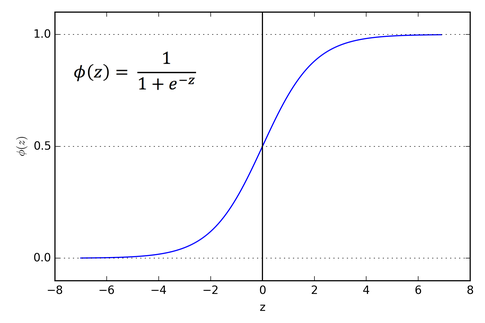
\includegraphics[width=0.7\textwidth]{img/4_marco_teorico/sigmoid_function.png}
    \label{fig:sigmoid_function}
    \begin{flushleft}
        \textit{Nota.} Extraído de \citet{farrukh_modeling_2019}. 
        \vspace{-\baselineskip}       
    \end{flushleft}
\end{figure}

Para \citet{hosmer2013applied} el método que busca estimar los valores óptimos de $\beta = (\beta_{0}, \beta_{1}, \beta_{2}, ..., \beta_{m})$ 
es la función de máxima verosimilitud, el cual se define como el producto de las probabilidades en las que cada instancia 
pertenece a la clase correcta:

\begin{equation}
    l(\beta) = \prod_{i=1}^{n} p_{i}^{y_{i}}(1 - p_{i})^{1 - y_{i}}
    \label{eq:likelihood}
\end{equation}

Para facilitar los cálculos, se trabaja con el logaritmo de la función de verosimilitud, conocido como log-verosimilitud:
\begin{equation}
    L(\beta) = \log l(\beta) = \sum_{i=1}^{n} y_{i} \log(p_{i}) + (1 - y_{i}) \log(1 - p_{i})
\end{equation}

Donde:
\begin{itemize}
    \item $L(\beta)$ es la función de verosimilitud
    \item $y_{i}$ es la etiqueta de clase de la observación $i$
    \item $p_{i}$ es la probabilidad predicha de la observación $i$
    \item $n$ es el número de observaciones
\end{itemize}

Los coeficientes $\beta$ que maximizan la log-verosimilitud, se obtienen derivando $L(\beta)$ 
con respecto a cada coeficiente $\beta_{j}$ e igualándolo a cero (Ecuación \ref{eq:partial_derivative}):

\begin{equation}
    \frac{\partial L(\beta)}{\partial \beta_{j}} = \sum_{i=1}^{n} (y_{i} - p_{i})X_{ij} = 0 \quad para \quad j = 0, 1, 2, ..., m
    \label{eq:partial_derivative}
\end{equation}

Donde:
\begin{itemize}
    \item $X_{ij}$ es el valor de la variable $j$ en la observación $i$
    \item $m$ es el número de variables predictoras
    \item $p_{i}$ es la probabilidad predicha de la observación $i$
    \item $n$ es el número de observaciones
    \item $y_{i}$ es la etiqueta de clase binaria de la observación $i$
    \item $\beta_{j}$ es el coeficiente de la variable $j$
    \item $L(\beta)$ es la función de log-verosimilitud
    \item $\partial L(\beta) / \partial \beta_{j}$ es la derivada parcial de la función de verosimilitud con respecto al coeficiente $\beta_{j}$
\end{itemize}

\paragraph{Entropía Cruzada Binaria (BCE).}
Según \citet{wali_xtreme_2022} para abordar problemas de clasificación binaria se utiliza la entropía cruzada binaria (BCE) como función
de pérdida, la cual mide la probabilidad de que un modelo asigne una clase correcta a la instancia, midiendo la disimilitud entre
las dos distribuciones de probabilidad. 

La probabilidad predicha está representada por un vector de probabilidades, donde la probabilidad predicha de la clase positiva se denota por $p$ 
y la probabilidad predicha de la clase negativa se denota por $1 -p$. La función 
de pérdida BCE se define la siguiente manera \citep{terven_loss_2024}:
\begin{equation}
    L(y, p) = -\frac{1}{N} \sum_{i=1}^{N} [y_i \log(p) + (1 - y_i) \log(1 - p)]
    \label{eq:binary_cross_entropy}
\end{equation}

El cual puede ser intuitivamente dividido en:
\[
\begin{cases}
    -\log(p) & \text{if  } y = 1 \\
    -\log(1 - p) & \text{if  } y = 0
\end{cases}
\]

Esta función de pérdida expresada como $-\log(x)$, como se visualiza en la Figura \ref{fig:cross_entropy}, convierte los valores en 
un rango de $[0, \infty)$.

\begin{figure}[H]
    \centering
    \caption{Función de pérdida de entropía cruzada binaria cuando la clase es positiva ($y = 1$)}
    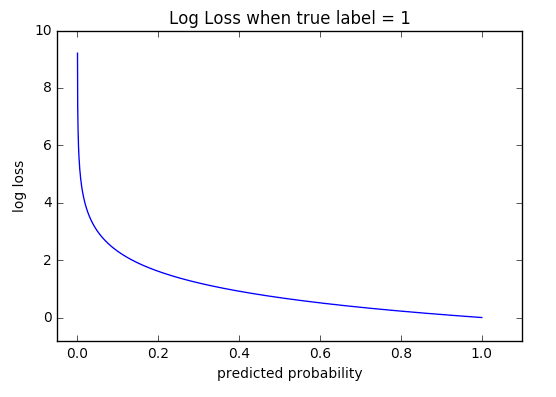
\includegraphics[width=0.7\textwidth]{img/4_marco_teorico/cross_entropy.png}
    \label{fig:cross_entropy}
    \begin{flushleft}
        \textit{Nota.} Extraído de \citet{machine_learning_glossary_loss_2017} 
        \vspace{-\baselineskip}       
    \end{flushleft}
\end{figure}

Este comportamiento es útil porque permite que la función de pérdida sea sensible a pequeñas diferencias en las probabilidades cercanas 
a 0 y 1, lo que es crucial en la clasificación. La entropía cruzada binaria penaliza fuertemente las predicciones incorrectas, acercando 
los valores de pérdida al infinito, mientras que las predicciones correctas reciben valores cercanos a 0. 

\paragraph{Entropía Cruzada Binaria Ponderada (WBCE).}
La entropía cruzada binaria es sensible al problema de desequilibrio de clases que ocurre
cuando el número de muestras de una clase es significativamente mayor que el de la otra. Para solucionar ello, se utiliza la entropía cruzada 
binaria ponderada para estos casos \citep{terven_loss_2024}.

En la entropía cruzada binaria ponderada (WBCE), se asigna un peso a cada muestra y la pérdida para cada muestra se calcula como:
\begin{equation}
    L(y, p) = -\frac{1}{N} \sum_{i=1}^{N} w_i[y_i \log(p) + (1 - y_i) \log(1 - p)]
    \label{eq:weighted_binary_cross_entropy}
\end{equation}

Donde $w_i$ es el peso asignado a la muestra $i$, $y$ es la etiqueta verdadera de clase binaria y $p$ es la probabilidad predicha para la clase positiva.
\citet{terven_loss_2024} sostiene que al asignar un mayor peso a las muestras de clases subrepresentadas, se alienta al modelo a prestar más atención a estas muestras y se puede mejorar el rendimiento general del modelo.

\paragraph{Función de pérdida de Dice.}
\citet{terven_loss_2024} define la función de pérdida de Dice como una medida de similitud entre la máscara de segmentación predicha y la máscara etiquetada para la clase positiva:

\begin{equation}
    DSC = 1 - \frac{2 \times |X \cap Y|}{|X| + |Y|}
    \label{eq:dice}
\end{equation}

Donde:
\begin{itemize}
    \item $X$ es la máscara de segmentación predicha
    \item $Y$ es la máscara de segmentación verdadera
    \item $|X \cap Y|$ es el número de píxeles en los que las máscaras de segmentación predicha y verdadera coinciden
    \item $|X|$ es el número de píxeles en la máscara de segmentación predicha
    \item $|Y|$ es el número de píxeles en la máscara de segmentación verdadera
\end{itemize}

\paragraph{WCE - Dice Loss.}
\citet{yali_evaluacion_2024} menciona que la combinación de múltiples funciones de pérdida es una estrategia viable para optimizar el rendimiento del modelo. 
En base a ello, formula la pérdida WCE-Dice que es una suma ponderada de las pérdidas 
de Entropía Cruzada Ponderada (WCE) y Dice (Ecuación \ref{eq:wbce_dice}).

\begin{equation}
    L_{WCE - Dice} = (1 -\alpha) \times L_{WCE} + \alpha \times L_{Dice}
    \label{eq:wbce_dice}
\end{equation}

Donde $\alpha$ es el coeficiente de ponderación (entre 0 y 1) que controla la importancia relativa de cada función de pérdida.

\paragraph{Árbol de decisión.}
\citet{Steinbach2004DataMC} definen el árbol de decisión como una estructura de datos jerárquica que toma decisiones dividiendo repetitivamente un conjunto de datos 
en subconjuntos más pequeños en función de reglas o condiciones basadas en características o atributos específicos. Los atributos utilizados en un árbol 
de decisión pueden ser nominales (categorías sin orden), ordinales (categorías con un orden inherente) o continuos (valores numéricos dentro de un rango definido). 

La estructura de un árbol de decisión se compone de nodos (Figura \ref{fig:decision_tree}), donde cada nodo representa una condición de prueba de un atributo y cada rama 
representa el resultado de dicha condición. Existen tres tipos de nodos: los nodos raíz, 
que son el punto de inicio del árbol y contienen la primera condición de prueba; los nodos internos, que representan condiciones de prueba subsecuentes y dividen los datos 
en función de los atributos; y los nodos hoja, que no se dividen más y representan las clases o valores de salida finales.

\begin{figure}[H]
    \centering
    \caption{Ejemplo de un árbol de decisión para un problema de clasificación de mamíferos.}
    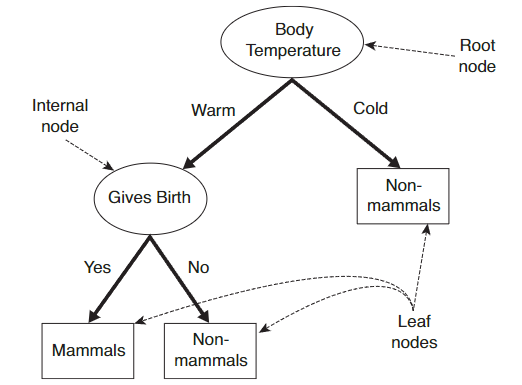
\includegraphics[width=0.7\textwidth]{img/4_marco_teorico/decision_tree.png}
    \label{fig:decision_tree}
    \begin{flushleft}
        \textit{Nota.} Extraído de \citet{Steinbach2004DataMC}. 
        \vspace{-\baselineskip}       
    \end{flushleft}
\end{figure}

Cada paso recursivo del proceso de construcción del árbol debe seleccionar una condición de prueba de atributos para dividir los registros en subconjuntos más pequeños hasta que todos los registros pertenezcan a la misma
clase o ya no exista ninguna ganancia en seguir dividiéndose.

Para implementar este paso, el algoritmo debe proporcionar un método para especificar la condición de prueba para
diferentes tipos de atributos, así como una medida objetiva para evaluar
la bondad de cada condición de prueba.

En cuanto al tipo de atributos, \citet{Steinbach2004DataMC} señalan que las condiciones de prueba para los atributos binarios generan divisiones binarias, mientras que los atributos nominales, ordinales y continuos pueden generar 
tanto divisiones binarias como multidireccionales (multiway), respetando en el caso de los ordinales su orden inherente y utilizando pruebas de comparación o consultas de rango para los continuos.

Para el crecimiento un árbol de decisión, existen muchas medidas que se pueden utilizar para determinar la mejor manera de dividir los registros. Estas se definen en términos 
de la distribución de clases de los registros antes y después de la división, siendo $p(i|t)$ la proporción de registros que pertenecen a la clase $i$ en el nodo $t$. 

En el caso de clasificación binaria, la distribución de 
clases en cualquier nodo se puede escribir como $(p_{0}, p_{1})$, donde $p_{1} = 1 − p_{0}$.

Las medidas desarrolladas para seleccionar la mejor división suelen basarse en el grado de impureza de los nodos secundarios, cuanto menor sea el grado de impureza, más sesgada será la 
distribución de clases. Por ejemplo, un nodo con una distribución de clases $(0, 1)$ tiene cero impurezas, mientras que un nodo con una distribución de clases uniforme $(0.5, 0.5)$ tiene la 
mayor impureza porque las clases están igualmente repartidas. Algunos ejemplos de medidas de impurezas se describen en \citet{Steinbach2004DataMC}:

\begin{subequations}
    \begin{gather}
        \text{Impureza de Gini} = 1 - \sum_{i=1}^{c} p_{i}^{2} \quad\\
        \text{Entropía} = -\sum_{i=1}^{c} p_{i} \log_{2}(p_{i}) \quad\\
        \text{Error de clasificación} = 1 - \max(p_{i})
    \end{gather}
\end{subequations}

Donde $c$ es el número de clases en el nodo y $p_{i}$ es la proporción de registros que pertenecen a la clase $i$ en el nodo específico. Los nodos con menor impureza presentan valores más bajos en estas medidas y, 
por lo tanto, se consideran mejores divisiones. La Figura \ref{fig:impurity} muestra cómo varían los valores de impureza según la proporción de clases para el índice de Gini, la entropía y el error de clasificación, 
donde las distribuciones más homogéneas $(p_{i} = 0.5)$ resultan en los valores máximos (0.5, 1, y 0.5 respectivamente) para cada medida.

\begin{figure}[H]
    \centering
    \caption{Comparación de las medidas de impureza de Gini, entropía y error de clasificación.}
    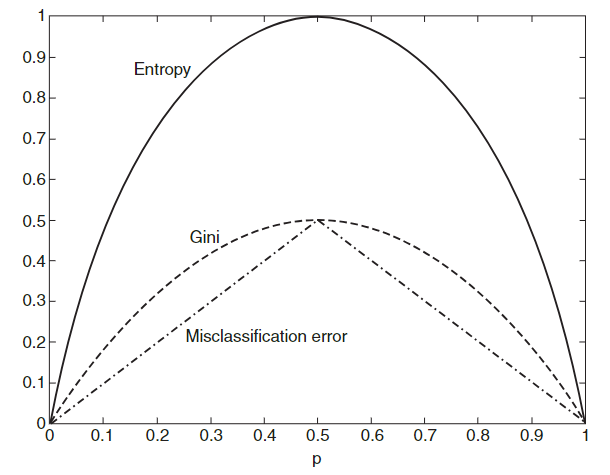
\includegraphics[width=0.5\textwidth]{img/4_marco_teorico/impureza.png}
    \label{fig:impurity}
    \begin{flushleft}
        \textit{Nota.} Extraído de \citet{Steinbach2004DataMC}. 
        \vspace{-\baselineskip}       
    \end{flushleft}
\end{figure}

Para determinar el rendimiento de una condición de prueba, necesitamos comparar el grado de impurezas del nodo padre (antes de la división) con el grado de impurezas de los nodos hijos (después de la división). 
Cuanto mayor sea la diferencia, mejor será la condición de prueba. 

La \textbf{ganancia} $(\Delta)$ es un criterio que se puede utilizar para determinar la bondad de una división:

\begin{equation}
    \Delta = I(parent) - \sum_{i=1}^{c} \frac{N(v_{i})}{N} \times I(v_{i})
    \label{eq:gain}
\end{equation}

Donde $I(parent)$ es la impureza del nodo padre, $N$ es el número total de registros en el nodo padre, $N(v_{i})$ es el número de registros en el nodo hijo $v_{i}$ y $I(v_{i})$ es la impureza del nodo hijo $v_{i}$.
Los algoritmos de inducción de árboles de decisión suelen elegir una condición de prueba que maximiza la ganancia $\Delta$. Dado que $I(parent)$ es el mismo para todas las condiciones de prueba, maximizar la ganancia es 
equivalente a minimizar las medidas de impureza promedio ponderadas de los nodos hijo. Cuando la entropía es utilizado como medida de impureza, la ganancia (diferencia entre entropías) se le conoce también como \textbf{ganancia de información} \citep{Steinbach2004DataMC}.

\paragraph{Gradient Boosting Decision Tree (GBDT).}
El GBDT, o árbol de decisión potenciado por gradiente, es un algoritmo de aprendizaje automático que utiliza boosting como técnica de ensamblado \citep{zhang_review_2022}. Según \citet{ke_lightgbm_2017}, este modelo entrena 
árboles de decisión en secuencia, ajustando en cada iteración los gradientes negativos, también conocidos como \textbf{errores residuales}.

Dado el conjunto de entrenamiento $D = \{X, Y\} = \{x_{j},y_{j}\}_{j=1}^N$, en donde $x_{j} \in R^c$ representa un vector predictivo de ``$c$'' características e 
$Y = \{y_j\}_{j=1}^N \in [0, 1]$ representa el conjunto de etiquetas de clases binarias para $N$ instancias, la finalidad del GBDT es encontrar una función objetivo $F(x)$ que prediga la etiqueta $Y$ 
para una nueva instancia de $X$. 

El entrenamiento inicia con un modelo simple, considerada como la hoja incial, que retorna un valor constante $F_{0}(X)$ que minimiza la función de pérdida en el conjunto de entrenamiento:

\begin{equation}
    F_0(X) = \text{argmin}_{\gamma} \sum_{j=1}^N L(y_j, \gamma)
\end{equation}

Posteriormente, para cada árbol $i = 1, 2, ..., m$ se calcula la función objetivo (donde $m$ es el máximo número de árboles definido) como se observa en la Figura \ref{fig:gbdt}.
\begin{figure}[H]
    \centering
    \caption{Ilustración de cómo trabaja el Gradient Boosting Tree.}
    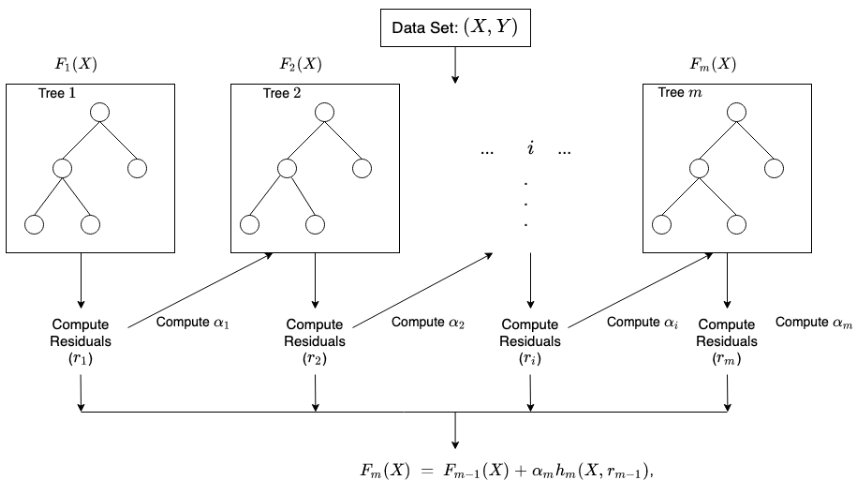
\includegraphics[width=0.9\textwidth]{img/4_marco_teorico/gradient_boost.png}
    \label{fig:gbdt}
    \begin{flushleft}
        \textit{Nota.} Extraído de \citet{amazon_web_services_how_2024}. 
        \vspace{-\baselineskip}       
    \end{flushleft}
\end{figure}

En cada nuevo árbol $i$, se calcula el error residual $r_{i}$ definido como la derivada de la función de pérdida con respecto a la función predictiva previa, esto se hace en el 
conjunto de entrenamiento o fracción dependiendo de la estrategia de muestreo utilizada (Ecuación \ref{eq:residuals}):
\begin{equation}
    r_{i} = -\left[\frac{\partial L(Y, F(X))}{\partial F(X)}\right]_{F(X)=F_{i-1}(X)}
    \label{eq:residuals}
\end{equation}

En este contexto, $F(X) = F_{i-1}(X)$ es la predicción del anterior modelo y $L(Y, F(X))$ es la función de pérdida diferenciable. 

Posteriormente, para predecir los \textbf{residuales} $r_{i}$ se entrena un nuevo árbol de decisión $(h_i)$, con un número máximo de hojas definido, que se agrega al modelo anterior $F_{i-1}(X)$.
Luego, se realiza una optimización de búsqueda de línea para determinar la tasa de aprendizaje $\alpha_i$ (Ecuación \ref{eq:learning_rate}): 

\begin{equation}
    \alpha_i h_{i}(X,r_{i-1}) = \text{argmin}_{\substack{\alpha, h}} \sum_{j=1}^N L(y_j, F_{i-1}(x_j) + \alpha_i h_i(x_j, r_{i-1}))
    \label{eq:learning_rate}
\end{equation}

Finalmente, se actualiza el modelo $F(X)$ con el nuevo árbol $h_i(X, r_{i-1})$ y se repite el proceso hasta que se alcance el número máximo de árboles $m$. 

\citet{mienye_survey_2022} definen a la función objetivo global, 
$F_{m}(x)$ como la suma ponderada de funciones:

\begin{equation}
    F_m(X) = F_{m-1}(X) + \alpha_m h_m(X, r_{m-1})
    \label{eq:funcion_objetivo}
\end{equation}

En donde $\alpha_m$ y $r_{m-1}$ son la tasa de aprendizaje (entre 0.01 a 1) y los residuales calculados para el árbol $m-1$ respectivamente, siendo $h_m$ el árbol de decisión que se entrena para predecir los 
residuales utilizando el conjunto de entrada $X$.

\paragraph{Algoritmo LightGBM.}
En el marco del Gradient Boosting Decision Tree, el algoritmo Light Gradient Boosting Machine (LightGBM) es una implementación eficiente del algoritmo de gradient boosting, desarrollada en 2017 
por investigadores de Microsoft. Este algoritmo se utiliza en problemas de clasificación, ranking y otros problemas de aprendizaje automático \citep{sun_forest_2022}.

\citet{ke_lightgbm_2017} desarrollaron el algoritmo LightGBM incorporando dos métodos innovadores: Gradient-based One-Sided Sampling (GOSS) y Exclusive Feature Bundling (EFB), que reducen el número de instancias y de características respectivamente, 
mejorando la eficiencia y velocidad del algoritmo al manejar datos de alta dimensionalidad y gran volumen. 

Asímismo, la construcción del árbol dentro del algoritmo se realiza mediante divisiones binarias asimétricas, con un número máximo de hojas predefinido, priorizando 
aquellas ramas que ofrecen la mayor ganancia de información \citep{ke_lightgbm_2017}.

En el \textbf{Gradient-based One-Sided Sampling (GOSS)} se conservan todos las instancias con gradientes grandes y realiza muestreo aleatorio en los ejemplos con gradientes pequeños ya que las instancias con grandes gradientes 
contribuirán mejor a la \textbf{ganancia de información}. Al reducir el muestreo de las instancias de datos, es preferible mantener aquellas con gradientes grandes y eliminar aleatoriamente solo aquellas 
con gradientes pequeños.

Para ello, LightGBM parte del algoritmo basado en histogramas. En este enfoque, los valores de las características se discretizan en k intervalos y se construye un histograma con un ancho de k (Figura \ref{fig:histogram}), durante el recorrido de los datos cada valor discretizado actúa 
como un índice en el histograma, lo que permite acumular estadísticas relevantes como la suma de gradientes. Una vez que se completa el primer recorrido de los intervalos, el histograma contiene las estadísticas necesarias, lo que permite un segundo recorrido para 
identificar el punto de división óptimo \citep{luo_two_2020}.

\begin{figure}[H]
    \centering
    \caption{Algoritmo basado en histogramas.}
    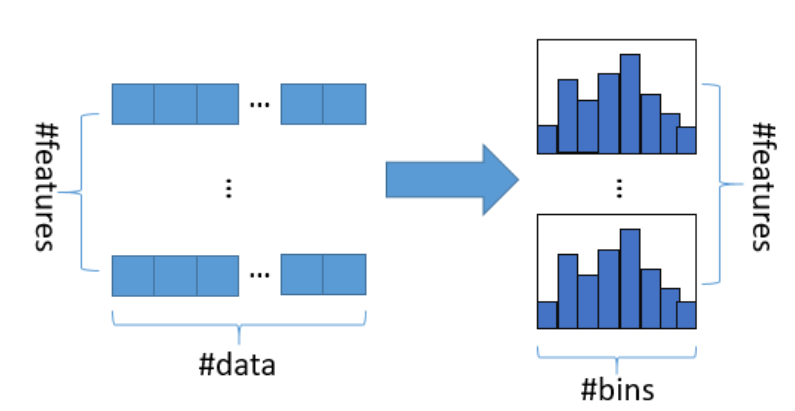
\includegraphics[width=0.7\textwidth]{img/4_marco_teorico/spliting.png}
    \label{fig:histogram}
    \begin{flushleft}
        \textit{Nota.} Extraído de \citet{luo_two_2020}. 
        \vspace{-\baselineskip}
    \end{flushleft}
\end{figure}

Esto se realiza para cada iteración de entrenamiento donde el modelo predice las etiquetas del conjunto de entrenamiento $I$ y calcula el gradiente de la función de pérdida $L$ para cada 
instancia $j$ en $I$. Posteriormente, se identifican como muestras de gran gradiente los primeros \(a \times 100\%\) de las muestras ordenadas por los valores absolutos de los gradientes de manera descendente, y las últimas \((1-a) 
\times 100\%\) se denominan muestras de pequeño gradiente, en donde $a$ y $b$ son las tasas de muestreo definidas como parámetro (Figura \ref{fig:goss}). 

De estas muestras de pequeño gradiente $(1 - a)$ se seleccionan de manera aleatoria una proporción de $b \times 100\%$ con un factor de peso
se inicializa con 1 para todas las instancias y se actualiza en cada iteración para ajustar los pesos de las instancias con gradientes pequeños \citep{ke_lightgbm_2017}.
\begin{figure}[H]
    \centering
    \caption{Pseucódigo del algoritmo Gradient-based One-Sided Sampling.}
    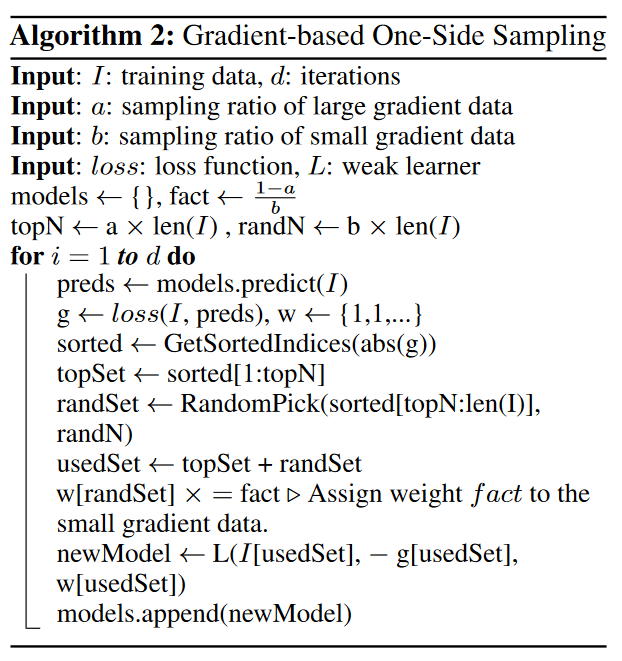
\includegraphics[width=0.5\textwidth]{img/4_marco_teorico/goss.png}
    \label{fig:goss}
    \begin{flushleft}
        \textit{Nota.} Extraído de \citet{ke_lightgbm_2017}. 
        \vspace{-\baselineskip}
    \end{flushleft}
\end{figure}

Por otro lado, el algoritmo \textbf{Exclusive Feature Bundling (EFB)} tiene la capacidad de agrupar numerosas características exclusivas en un conjunto mucho más pequeño de características densas. Este proceso de agrupamiento reduce significativamente 
los cálculos innecesarios para los valores nulos. 

De esta manera, la complejidad de construcción del histograma cambia de $O(\text{datos} \times \text{características})$ a $O(\text{datos} \times \text{grupo})$, siendo $\text{\# grupo} \ll \text{\# característica}$. Para ello, lo primero
que debe determinarse es que caracterísiticas deben agruparse juntas a través del método \textbf{Greedy Bundling} y lo segundo es unir las características con el método \textbf{Merge Exclusive Features} como se 
muestra en forma de pseudocódigo en la Figura \ref{fig:efb} \citep{ke_lightgbm_2017}.

\begin{figure}[H]
    \centering
    \caption{Pseucódigo del método Exclusive Feature Bundling.}
    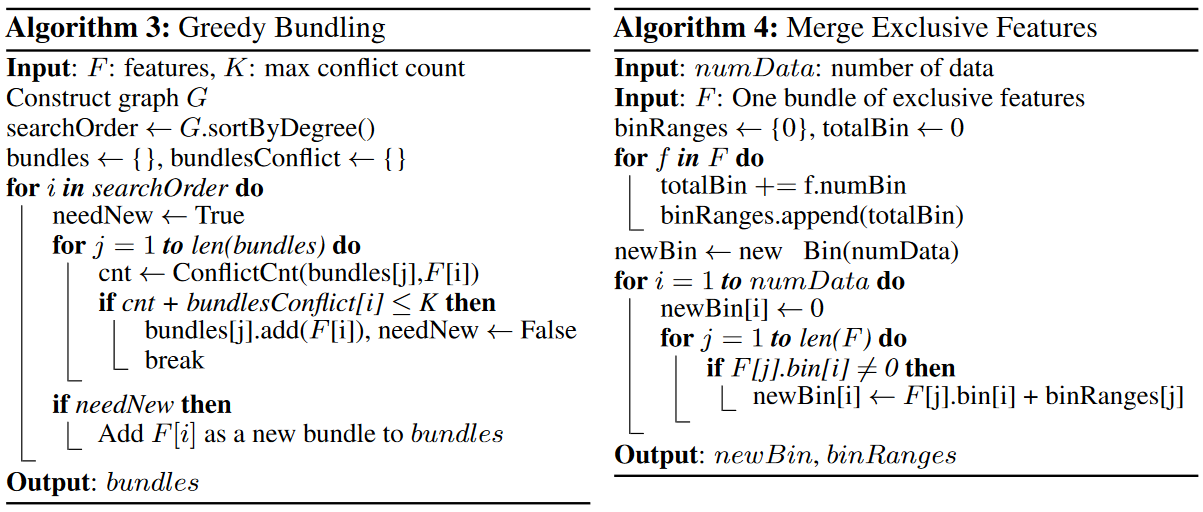
\includegraphics[width=1\textwidth]{img/4_marco_teorico/efb.png}
    \label{fig:efb}
    \begin{flushleft}
        \vspace{-\baselineskip}
        \textit{Nota.} Extraído de \citet{ke_lightgbm_2017}. 
        \vspace{-\baselineskip}
    \end{flushleft}
\end{figure}

El método denominado \textbf{Greedy Bundling} tiene como objetivo agrupar las características 
en pares capturando la mayor cantidad de instancias exclusivas, es decir aquellas instancias 
donde uno de los valores es cero y el otro no \citep{meanxai_mxml-12-03_2023}  

En la Figura \ref{fig:greddy} se observa cómo el método comienza con un conjunto de características $F_{0}, F_{1}, ..., F_{4}$ y un conjunto de instancias $i_{0}, i_{1}, ..., i_{9}$. Al realizar el grafo correspondiente $G$ se capturan las 
instancias que generan conflicto, es decir que no son exclusivas, para cada par de características.

Luego, se suma el número de conflictos entre cada par de características y se ordena de manera descendente (searchOrder).
Después, se inicia con la primera característica en ``searchOrder'' y se procede a agrupar las características bajo la condición de que el número máximo de conflictos entre características sea menor o igual a $K$. 
En este caso, con $K = 1$ se obtienen tres grupos o bundles: $F_4, F_{0-3}, F_{1-2}$.

\begin{figure}[H]
    \centering
    \caption{Ejemplo de cómo trabaja el Greedy Bundling - EFB.}
    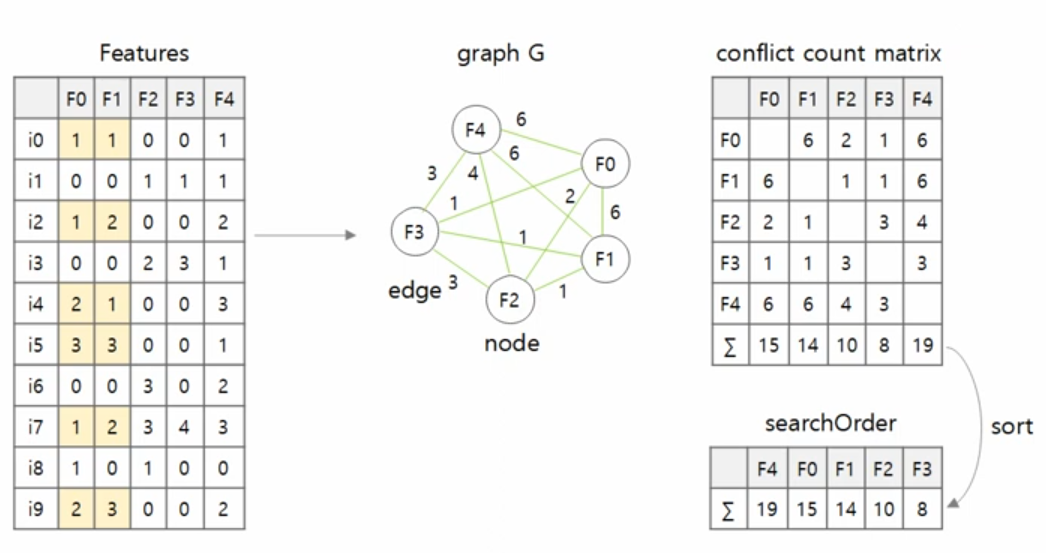
\includegraphics[width=0.7\textwidth]{img/4_marco_teorico/efb2.png}
    \label{fig:greddy}
    \begin{flushleft}
        \textit{Nota.} Extraído de \citet{meanxai_mxml-12-03_2023}. 
        \vspace{-\baselineskip}
    \end{flushleft}
\end{figure}

En \citet{meanxai_mxml-12-03_2023}, utilizando el método \textbf{Merge Exclusive Features} (Figura \ref{fig:merge_exclusive_features}) se combinan los grupos en una única característica priorizando las instancias. Cuando la instancia de la característica 
no es igual a cero, $F \times bin \neq 0$, se suma el valor de la instancia en la característica con el correspondiente $binRanges$ obtenido del acumulado del rango de los máximos valores de cada característica. 
\begin{figure}[H]
    \centering
    \caption{Ejemplo de cómo trabaja el Merge Exclusive Features.}
    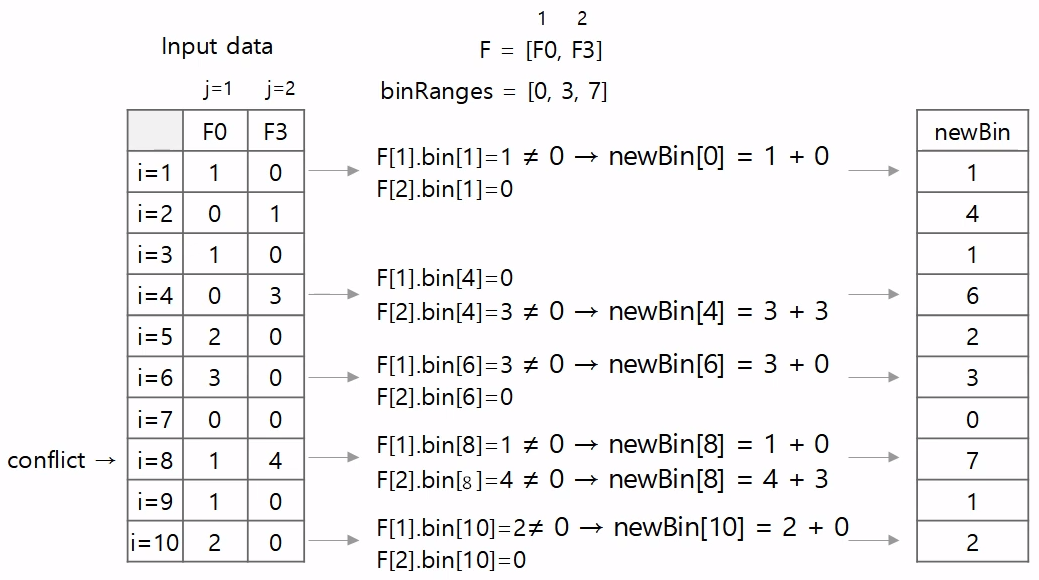
\includegraphics[width=0.6\textwidth]{img/4_marco_teorico/merge_exclusive_features.png}
    \label{fig:merge_exclusive_features}
    \begin{flushleft}
        \textit{Nota.} Extraído de \citet{meanxai_mxml-12-03_2023}. 
        \vspace{-\baselineskip}
    \end{flushleft}
\end{figure}

\subsection{Segmentación Semántica}
La segmentación semántica desempeña un papel fundamental en una amplia variedad de aplicaciones de visión por computadora, proporcionando información clave para la comprensión global de una imagen. 
En términos concretos, su objetivo es etiquetar los píxeles de la imagen con las clases semánticas correspondientes y proporcionar límites de las clases de objetos, facilitando la comprensión de las apariencias de los objetos y las relaciones espaciales entre ellos.
\citep{csurka2023semantic}

\begin{figure}[H]
    \centering
    \caption{Ejemplo de segmentación semántica.}
    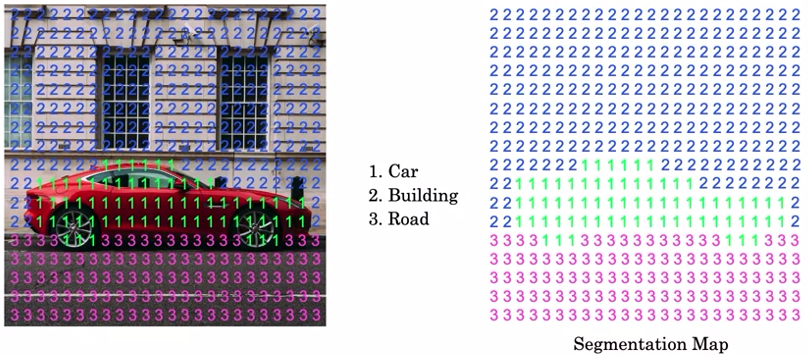
\includegraphics[width=0.8\textwidth]{img/4_marco_teorico/segmentation.png}
    \label{fig:semantic_segmentation}
    \begin{flushleft}
        \textit{Nota.} Extraído de \citet{ng_semantic_2023}. 
        \vspace{-\baselineskip}       
    \end{flushleft}  
\end{figure}

\subsubsection{Red Neuronal Convolucional (CNN).}
\citet{balas_recent_2020} lo definen como un tipo de red neuronal artificial (ANN) con una arquitectura de retroalimentación profunda que le permite aprender diversas características de los objetos, 
especialmente características espaciales. Las capas iniciales de un modelo CNN aprenden y extraen las características de alto nivel con una abstracción más baja y las capas más 
profundas aprenden y extraen las características de bajo nivel con mayor abstracción.

\citet{katsaros_backpropagation_2021} menciona que una CNN es apropiada para procesar entradas tipo cuadrícula 
como imágenes, videos y series de tiempo. Asímismo, su menor número de parámetros entrenables en comparación con una red neuronal artificial (ANN) convencional ayuda a reducir el riesgo de 
sobreajuste y mejora la capacidad de generalización del modelo \citep{balas_recent_2020}.

\subsubsection{Arquitectura U-Net.}
Según \citet{al_dabbagh_2023}, la arquitectura U-Net está diseñada específicamente para la tarea de segmentación semántica una forma de U y que consta de rutas de contracción (codificador) en el lado izquierdo y rutas expansivas,
siendo un ejemplo típico de un modelo que consta de capas de convolución y agrupación.

\paragraph{Capa convolucional.}
La capa convolucional es considerada la parte principal de la CNN, contiene un conjunto de núcleos, también llamado filtros o kernel que convolucionan con la imagen de entrada  
para generar como resultado un mapa que abstrae las características relevantes de la imagen. Un núcleo puede describirse como una cuadrícula de valores o pesos que pueden ser aleatorios 
o inicializados.

Una operación convolucional se define como el producto punto entre el núcleo y la imagen de entrada, donde se multiplican los valores correspondientes de ambos y se suman todos los productos resultantes 
para generar un valor escalar en el mapa de características (Figura \ref{fig:convolutional_layer}). Este proceso se realiza de manera sistemática a medida que el núcleo se desliza sobre la imagen de entrada en pasos definidos, conocidos 
como strides.

\begin{figure}[H]
    \centering
    \caption{Ilustración de los primeros cinco pasos en una operación de convolución para una imagen de entrada 4x4x1 y un núcleo de 2x2.}
    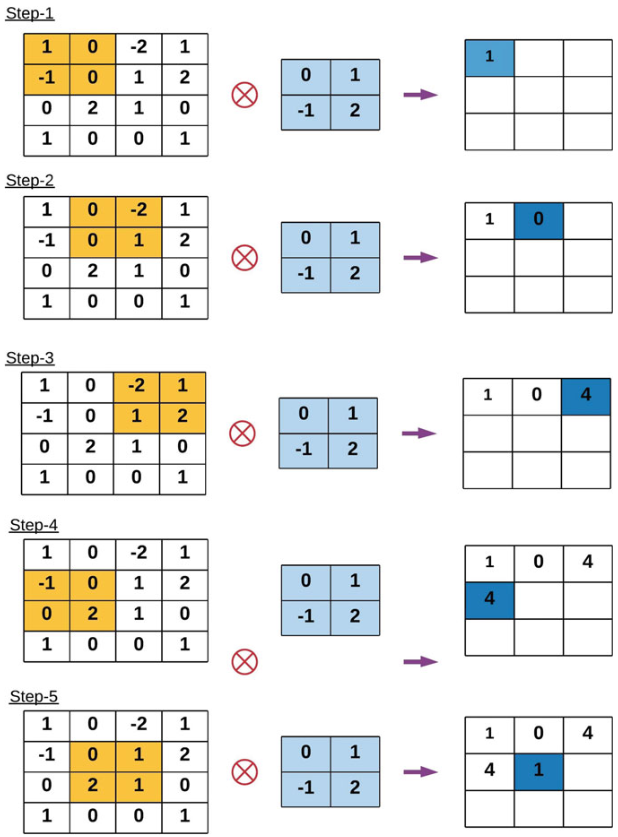
\includegraphics[width=0.4\textwidth]{img/4_marco_teorico/convolutional_layer.png}
    \label{fig:convolutional_layer}
    \begin{flushleft}
        \textit{Nota.} Extraído de \citet{balas_recent_2020}. 
        \vspace{-\baselineskip}       
    \end{flushleft}
\end{figure}

En la Figura \ref{fig:feature_map}, \citet{Goodfellow-et-al-2016} muestran una versión generalizada de la operación de convolución en donde el núcleo (Kernel) se desliza sobre la imagen de entrada para generar un mapa de características.
El resultado en cada pixel del mapa de características se obtiene mediante el producto punto, es decir la suma de los productos de los elementos correspondientes a la región de la imagen de entrada (Input) cubierta por el núcleo y el núcleo mismo.

\begin{figure}[H]
    \centering
    \caption{Mapa de característica resultante después de una operación de convolución 2\times2.}
    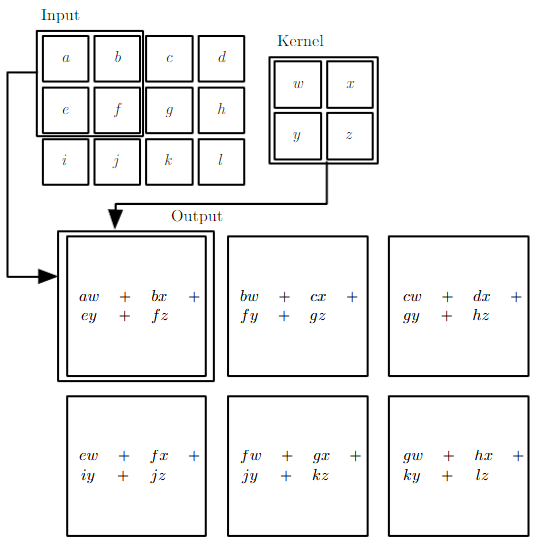
\includegraphics[width=0.4\textwidth]{img/4_marco_teorico/feature_map.png}
    \label{fig:feature_map}
    \begin{flushleft}
        \textit{Nota.} Extraído de \citet{Goodfellow-et-al-2016}. 
        \vspace{-\baselineskip}       
    \end{flushleft}
\end{figure}

\paragraph{Padding y Stride.}
El relleno o padding es crucial para preservar la información en los bordes de la imagen de entrada durante la convolución. Sin el uso de relleno, las características situadas en los bordes de la imagen se pueden perder 
rápidamente a medida que el núcleo de convolución no puede abarcar completamente estas regiones. 

El relleno se utiliza para aumentar el tamaño de la imagen de entrada, lo que a su vez incrementa el tamaño del mapa de 
características de salida. Esto permite que todas las características, incluidas las de los bordes, se consideren en el proceso de convolución, manteniendo así más información relevante de la imagen original.

Por otro lado, las zancadas, pasos o stride son la cantidad de píxeles que se mueve el núcleo en cada paso de la convolución. La fórmula generalizada para calcular el tamaño del mapa de características de salida utilizando 
\textbf{padding y stride} se detalla en \citet{balas_recent_2020}:

\begin{subequations}
    \begin{gather}
        h^{'} = \frac{h- f + 2p}{s} + 1 \\
        w^{'} = \frac{w- f + 2p}{s} + 1        
    \end{gather}
    \label{eq:feature_map_size}
\end{subequations}

Donde $h^{'}$ y $w^{'}$ denotan la altura y ancho del mapa de características de salida, $h$  y $w$ denotan la altura y ancho de la imagen de entrada, 
$f$ es el tamaño del filtro, $p$ es el relleno de la operación de convolución y $s$ la zancada en la operación de convolución.

Se tiene el siguiente ejemplo para una operación de convolución utilizando un padding de 1 (relleno de ceros)
y un stride de 3 (Figura \ref{fig:padding_stride}); siguiendo con los cálculos de la Ecuación \ref{eq:feature_map_size} se tiene un mapa de características 
de salida con dimensiones de $2\times2$.
\begin{figure}[H]
    \centering
    \caption{Ejemplo de una operación de convolución utilizando un padding de 1 y un stride de 3.}
    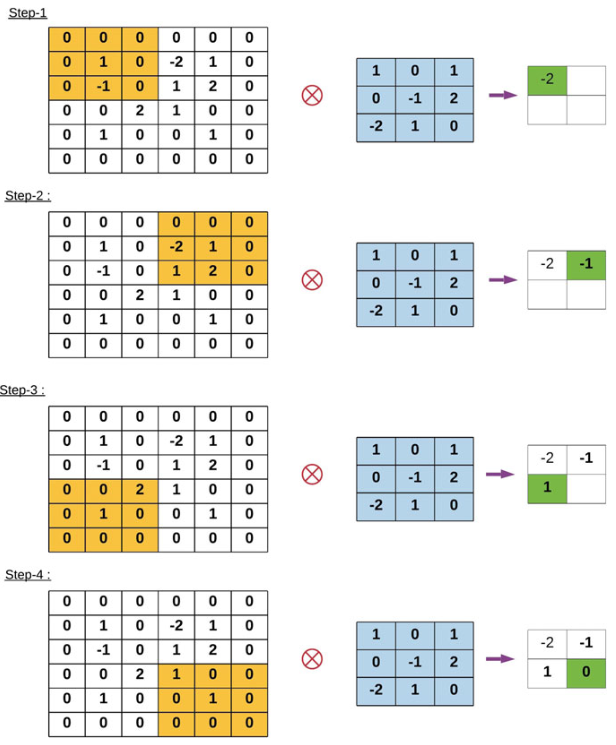
\includegraphics[width=0.5\textwidth]{img/4_marco_teorico/padding_stride.png}
    \label{fig:padding_stride}
    \begin{flushleft}
        \textit{Nota.} Extraído de \citet{balas_recent_2020}. 
        \vspace{-\baselineskip}       
    \end{flushleft}    
\end{figure}

\paragraph{Funciones de activación.}
En la arquitectura CNN, después de cada capa con parámetros, se utilizan capas de activación no lineal. 
El comportamiento no lineal de esas capas permite que el modelo CNN aprenda cosas más complejas y logre asignar las entradas a las salidas de forma no lineal. \citet{balas_recent_2020} 
mencionan que las funciones de activación más utilizada en redes neuronales profundas es la función ReLU (Rectified Linear Unit) (Ecuación \ref{eq:relu}).
\begin{equation}
    f(x) = max(0,x)
    \label{eq:relu}
\end{equation}

La función ReLU (Figura \ref{fig:relu}) activa solo los valores positivos y deja los negativos como cero, lo que introduce la no linealidad necesaria y acelera la convergencia del entrenamiento.
\begin{figure}[H]
    \centering
    \caption{Función de activación ReLU.}
    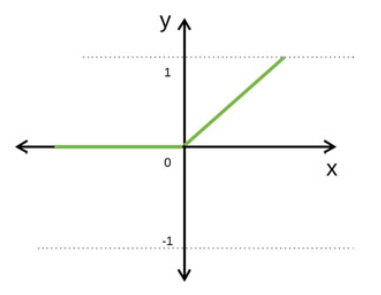
\includegraphics[width=0.5\textwidth]{img/4_marco_teorico/relu_function.png}
    \label{fig:relu}
    \begin{flushleft}
        \textit{Nota.} Extraído de \citet{balas_recent_2020}. 
        \vspace{-\baselineskip}       
    \end{flushleft}  
\end{figure}

\paragraph{Capa de agrupación.}
La capa de agrupación o pooling layer se utiliza para submuestrear los mapas de características producidos después de operaciones de convolución,
es decir toma un mapa de características de entrada y reduce su tamaño conservando las características más dominantes en cada stride del grupo. 

Existen diferentes tipos de técnicas de agrupación: agrupación máxima, mínima, promedio, cerrada, etc. De entre ellas, el max pooling es el método 
más popular y utilizado.

La fórmula para encontrar el tamaño del mapa de características de salida después de la operación de agrupación es:
\begin{subequations}
    \begin{gather}
        h^{'} = \frac{h - f}{s} + 1 \\
        w^{'} = \frac{w - f}{s} + 1
        \label{eq:pooling_size}
    \end{gather}
\end{subequations}

Donde $h^{'}$ y $w^{'}$ denotan la altura y ancho del mapa de características de salida, $h$  y $w$ denotan la altura y ancho de la imagen de entrada, 
$f$ es el tamaño del filtro y $s$ la zancada en la operación de convolución.

\citet{balas_recent_2020} ejemplifican la operación de max pooling en una imagen de $4\times4$ con un filtro de $2\times2$ al cual 
da como resultado un mapa de caracterísiticas de dimensiones $3\times3$ (Figura \ref{fig:max_pooling}). 
\begin{figure}[H]
    \centering
    \caption{Ejemplo de una operación de max pooling utilizando un stride de 1 y un tamaño de filtro de $2\times2$.}
    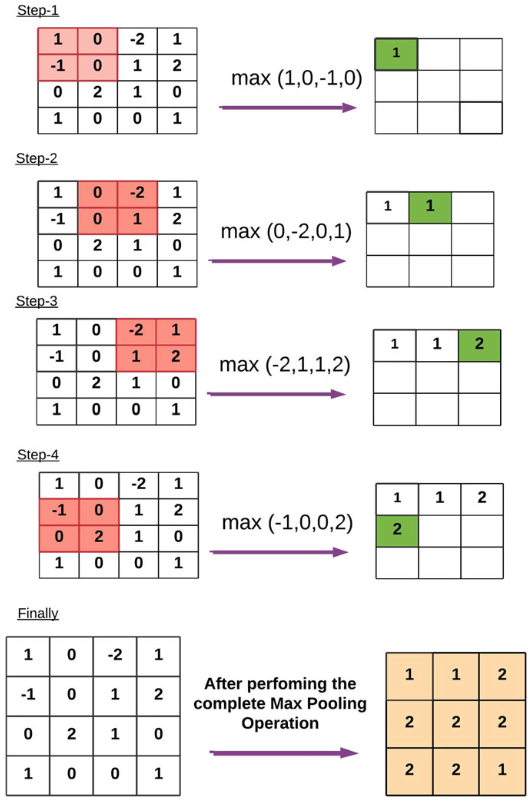
\includegraphics[width=0.5\textwidth]{img/4_marco_teorico/max_pooling.png}
    \label{fig:max_pooling}
    \begin{flushleft}
        \textit{Nota.} Extraído de \citet{balas_recent_2020}. 
        \vspace{-\baselineskip}       
    \end{flushleft}  
\end{figure}

\paragraph{Capa de Deconvolución.}
\citet{somukesh_apply_2023} define la capa de deconvolución como la capa que utiliza la operación de convolución transpuesta para aumentar la resolución espacial de una imagen. 

A diferencia de la convolución estándar, la deconvolución expande el tamaño de la entrada al aplicar un filtro que redistribuye los valores del mapa de características de entrada a una salida más 
grande. Una operación de deconvolución se puede definir como un proceso donde un filtro o núcleo deconvolucional se aplica a cada valor de la entrada, esparciendo estos valores sobre la salida de acuerdo 
con los pesos del filtro. En cada paso, el núcleo multiplica los valores de entrada por sus pesos correspondientes y distribuye el resultado en la posición correspondiente de la salida.

En la Figura \ref{fig:deconvolution_example}, se ilustra cómo funciona la deconvolución con una entrada de $2 \times 2$, un filtro de $2 \times 2$ y un stride de 1. Para cada valor de la entrada, el filtro 
se aplica y se suma al mapa de salida en todas las posiciones afectadas. 

Este proceso resulta en un mapa de características de salida de mayor tamaño, en este caso $3 \times 3$, donde cada valor representa la 
acumulación de las multiplicaciones ponderadas de los valores de entrada y los pesos del filtro.

\begin{figure}[H]
    \centering
    \caption{Ilustración de los pasos en una operación de deconvolución para una entrada de 2x2 y un núcleo de 2x2 con un stride de 1.}
    \label{fig:deconvolution_example}
    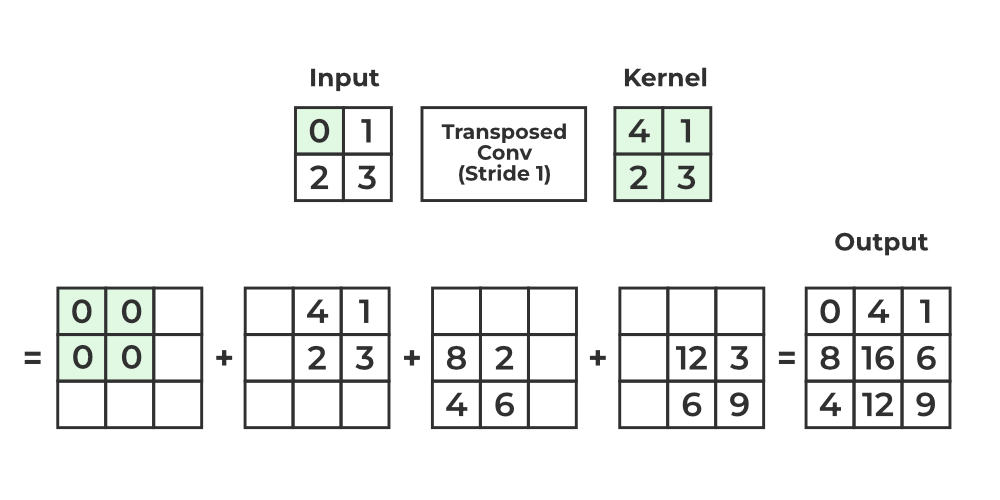
\includegraphics[width=0.8\textwidth]{img/4_marco_teorico/upconv.png}
    \begin{flushleft}
        \vspace{-\baselineskip}
        \textit{Nota.} Extraído de \citet{somukesh_apply_2023}.
        \vspace{-\baselineskip}  
    \end{flushleft}
\end{figure}

Las dimensiones del mapa de características de salida se pueden calcular utilizando la siguiente fórmula descrita en \citet{somukesh_apply_2023}:

\begin{subequations}
    \begin{gather}
        h^{'} = s(h-1) + f - 2p + k \\
        w^{'} = s(w-1) + f - 2p + k
        \label{eq:deconvolution_size}
    \end{gather}
\end{subequations}

Donde $h^{'}$ y $w^{'}$ denotan la altura y ancho del mapa de características de salida, $h$  y $w$ denotan la altura y ancho de la imagen de entrada,
$f$ es el tamaño del filtro, $p$ es el relleno de la operación de deconvolución, $s$ la zancada en la operación de convolución y $k$ el tamaño del kernel.

\paragraph{Función de costo.}
Para \citet{balas_recent_2020} la función de costo $J$, se define como el promedio de la función de pérdida de entropía cruzada sobre todas las muestras de entrenamiento. Esta función de costo se expresa como:
\begin{equation}
    J = \frac{1}{N} \sum_{i=1}^{N} L_i
    \label{eq:cost_function}
\end{equation} 
Donde:
\begin{itemize}
    \item $J$ es la función de costo.
    \item $L_i$ es la función de pérdida de la muestra $i$.
    \item $N$ es el número total de muestras de entrenamiento.
\end{itemize}

\paragraph{Codificador y Decodificador.}
En la Figura \ref{fig:u-net} se ilustran los dos componentes principales de la arquitectura U-Net: el codificador (encoder) y el decodificador (decoder).

Según \citet{ronneberger_2015}, la arquitectura de la U-Net está estructurada en dos trayectorias principales: una ruta de contracción, conocida como codificador, 
situada en el lado izquierdo y una ruta de expansión, llamada decodificador, ubicada en el lado derecho.

La ruta de contracción sigue la arquitectura clásica de una red convolucional, donde se aplican de forma repetida dos convoluciones de $3 \times 3$ (sin relleno), 
cada una seguida de una función de activación ReLU, y una operación de max-pooling de $2 \times 2$ con un paso de 2 para disminuir la resolución espacial. 

En la ruta de expansión, cada paso comienza con un aumento de la resolución espacial del mapa de características mediante una convolución transpuesta de $2 \times 2$ 
(up-conv), que también reduce a la mitad el número de canales de características. Este mapa de características aumentado se concatena con el correspondiente mapa de 
características de la ruta de contracción, que ha sido recortado para alinearse espacialmente. Por último, se aplican dos convoluciones de $3 \times 3$, cada una seguida 
de una ReLU, para obtener el mapa de características final de la segmentación.

\begin{figure}[H]
    \centering
    \caption{Arquitectura U-Net de un modelo de red neuronal convolucional.}
    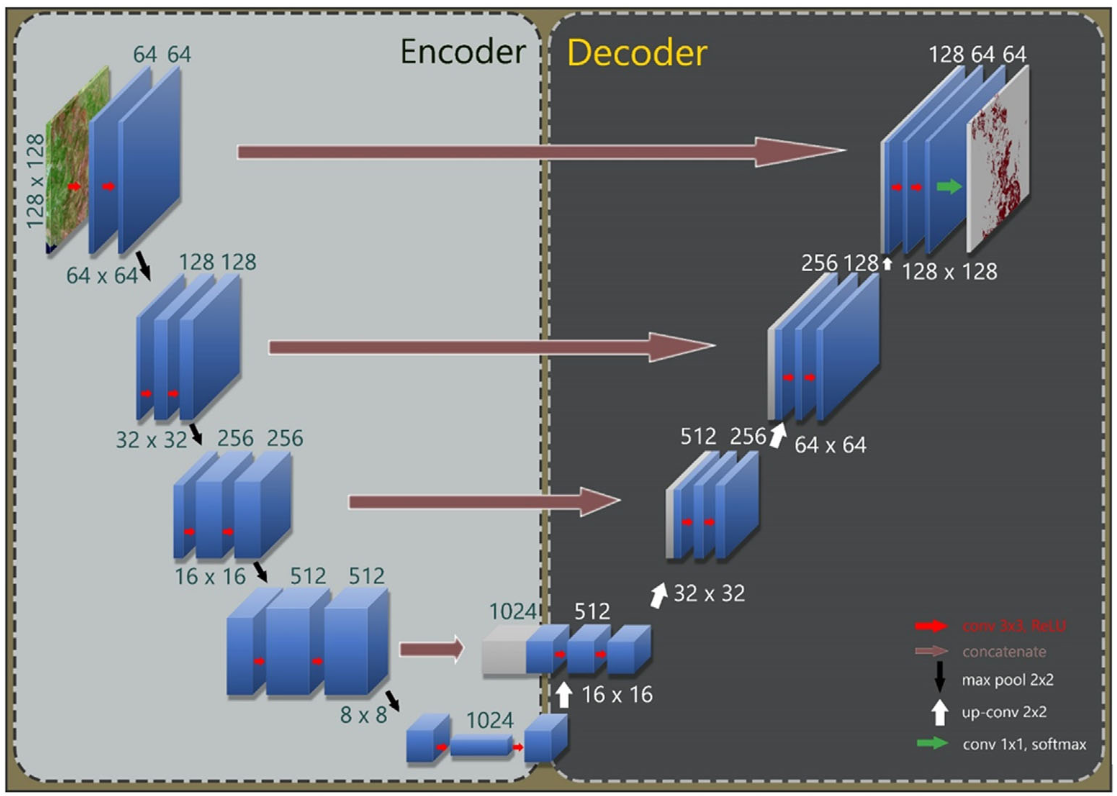
\includegraphics[width=0.7\textwidth]{img/4_marco_teorico/u_net.png}
    \label{fig:u-net}
    \begin{flushleft}
        \textit{Nota.} Extraído de \citet{al_dabbagh_2023}. 
        \vspace{-\baselineskip}       
    \end{flushleft}  
\end{figure}

\subsubsection{Hiperparámetros del entrenamiento de una CNN.}
\citet{wei_understanding_2024} define a los siguientes hiperparámetros de entrenamiento como los que controlan el proceso de entrenamiento de la red neuronal 
convolucional:
\begin{itemize}
    \item Tasa de aprendizaje: Regula el tamaño del paso que el optimizador da al ajustar los pesos de la red en cada iteración. Una tasa de aprendizaje 
    alta puede acelerar el entrenamiento, pero corre el riesgo de saltar sobre mínimos locales.
    \item Número de épocas: Indica cuántas veces el modelo verá el conjunto de entrenamiento completo. Más épocas pueden permitir un mejor ajuste, pero 
    también pueden llevar a sobreajuste.
    \item Tamaño del lote: Es la cantidad de muestras del dataset en un lote (batch) que se utilizan en cada iteración del entrenamiento.
    \item Iteraciones: El número de actualizaciones de pesos que se realizan en una época. Se calcula como el número de muestras dividido por el tamaño del lote.
    \item Número de filtros: Cantidad de filtros que se aplican en cada capa convolucional.
    \item Número de capas: Cantidad de capas convolucionales y de agrupación que se utilizan en la red.
\end{itemize}

\subsection{Métricas de evaluación}
\label{sec:metricas_evaluacion}
Los métodos de evaluación en la segmentación semántica tienen como objetivo calificar la similitud entre la segmentación predicha y la etiqueta real (ground truth). Aunque existen numerosas métricas de evaluación en la literatura, solo 
algunas se han demostrado apropiadas y se utilizan de manera estandarizada \citep{muller_towards_2022}.

Todas las métricas presentadas se basan en la computación de una matriz de confusión para una tarea de segmentación, la cual 
contiene el número de verdaderos positivos (VP), falsos positivos (FP), verdaderos negativos (VN) y falsos negativos (FN). En donde 
los rangos de valor de todas las métricas presentadas oscilan entre cero (peor) y uno (mejor).

\subsubsection{Métricas basadas en F-measure.}
Las métricas basadas en F-measure, también conocidas como puntuaciones F, son una de las puntuaciones más extendidas para medir el 
rendimiento en visión por computadora. Se calculan a partir de la sensibilidad y precisión de una predicción, lo que evalúa la 
superposición entre la segmentación predicha y el ground truth. Aún así, al incluir la precisión, penalizan los falsos positivos, 
un factor común en conjuntos de datos altamente desequilibrados en clases. 

Dos métricas populares utilizadas basadas en F-measure son el Índice de Intersección sobre Unión (IoU en Ecuación \ref{eq:iou}) y el coeficiente de similitud de Dice o $F_1$ en la Ecuación \ref{eq:f1}. 
\begin{equation}
    IoU = \frac{TP}{TP + FP + FN}
    \label{eq:iou}
\end{equation}

\begin{equation}
    F_1 = \frac{2 \times TP}{2 \times TP + FN + FP}
    \label{eq:f1}
\end{equation}

A pesar de que el IoU penaliza más la sub-segmentación y sobre-segmentación que el $F_1$, ambos son métricas adecuadas y las más utilizadas en el 
campo de la observación de la Tierra \citep{arnaudo_robust_2023,cabuar_2023,al_dabbagh_2023}

\subsubsection{Sensibilidad y Especificidad.}
La sensibilidad y especificidad son métricas estándar establecidas para la evaluación del rendimiento. 

La sensibilidad o Precision en la Ecuación \ref{eq:precision} se centra en la 
capacidad de detección de verdaderos positivos, mientras que la especificidad o Recall en la Ecuación \ref{eq:recall} evalúa la capacidad de identificar correctamente las clases verdaderas negativas.

\begin{equation}
    Precision = \frac{TP}{TP + FP}
    \label{eq:precision}
\end{equation}

\begin{equation}
    Recall = \frac{TP}{TP + FN}
    \label{eq:recall}
\end{equation}

\subsubsection{Precisión o Índice Rand.}
La Precisión o Accuracy, también conocida como índice Rand, es una de las métricas más conocidas en estadística. Sin embargo, 
su uso está fuertemente desaconsejado en EO porque las imágenes de segmentación semántica suelen estar altamente desequilibradas en clases. 
Debido a la inclusión de verdaderos negativos (TN), esta métrica de precisión siempre dará puntuaciones muy altas de manera ilegítima \citep{muller_towards_2022}.

\begin{equation}
    Accuracy = \frac{TP + TN}{TP + TN + FP + FN}
    \label{eq:accuracy}
\end{equation}

\subsubsection{Índice Kappa.}
El Índice Kappa de Cohen (\(\kappa\)) para clasificación binaria se define como:
\[\kappa = \frac{P_o - P_e}{1 - P_e}\]

Donde:
\begin{itemize}
  \item \(P_o\) es la proporción de acuerdo observado entre los clasificadores.
  \item \(P_e\) es la proporción de acuerdo esperado por azar.
\end{itemize}


\citet{foody_explaining_2020} menciona que para el caso simple de una matriz de confusión binaria, la proporción de acuerdo, $P_{o}$ y $P_{e}$, 
se estiman de la siguiente forma:

\begin{itemize}
  \item La proporción de acuerdo observado (\(P_o\)) se calcula como:
  \[  P_o = \frac{TP + TN}{TP + FP + FN + TN} \]
  \item La proporción de acuerdo esperado por azar (\(P_e\))  basado en los márgenes de la matriz de confusión se calcula como:
  \[P_e = \frac{(TP + FP) \cdot (TP + FN) + (FN + TN) \cdot (FP + TN)}{(TP + FP + FN + TN)^2} \]
\end{itemize}

\subsubsection{Curva ROC y Área Bajo la Curva (AUC).}
La curva ROC (Receiver Operating Characteristic) es una representación gráfica que muestra la tasa de verdaderos positivos (TVP) frente a la tasa de falsos positivos (TFP) 
para diferentes umbrales de discriminación. 

El área bajo la curva ROC (AUC) es una métrica común para validar clasificadores de aprendizaje automático. Un AUC de 0.5 indica 
un clasificador aleatorio, mientras que valores cercanos a 1 indican un mejor rendimiento. 

La fórmula del AUC se define como el área del trapecio según \citet{DBLP:journals/corr/abs-2010-16061}.
\begin{equation}
    \text{AUC} = 1 - (\frac{fpr + tpr}{2})
    \label{eq:auc}
\end{equation}

La tasa de verdaderos positivos (TVP) y la tasa de falsos positivos (TFP) se calculan como:

\begin{equation}
    \text{TVP} = \frac{\text{TP}}{\text{TP} + \text{FN}}
    \label{eq:tvp}
\end{equation}

\begin{equation}
    \text{TFP} = \frac{\text{FP}}{\text{FP} + \text{TN}}
    \label{eq:tfp}
\end{equation}

En donde:
\begin{itemize}
    \item TP = Verdaderos positivos.
    \item TN = Verdaderos negativos.
    \item FP = Falsos positivos.
    \item FN = Falsos negativos
\end{itemize}

\subsection{Quema de caña de azúcar}

\subsubsection{Fenología de la caña de azúcar.}
% Definir la caña de azúcar, su cultivo y morfología

Según \citet{helfgott_cultivo_2016}, la caña de azúcar, con nombre científico \textit{Saccharum officinarum}, es una planta perenne de la familia de las gramíneas, originaria de Asia tropical 
y subtropical que se adapta bien a una variedad de suelos, siempre y cuando haya disponibilidad de agua, aunque prefiere las temperaturas tropicales y suelos de 
textura franca, con un pH cercano a 7.0, bien drenados y profundos. 

El ciclo vegetativo de la caña de azúcar se desarrolla en las siguientes fases:
\begin{enumerate}
    \item \textbf{Pre-brotamiento:} Desde el tapado de la semilla vegetativa (estaca) o desde la cosecha, hasta el inicio del brotamiento de las yemas.
    \item \textbf{Brotamiento:}  Desde el inicio del brotamiento de las yemas hasta el surgimiento de las raíces.
    \item \textbf{Enraizamiento:} Durante esta fase, se desarrollan las raíces permanentes del brote.
    \item \textbf{Macollaje:} Durante este período, se forman los vástagos o tallos de la caña. Esta etapa comienza entre 20 y 40 días después de la siembra o corte.
    \item \textbf{Etapa inicial de crecimiento:} Durante esta fase, se forman los entrenudos y aumenta el sistema radicular permanente.
    \item \textbf{Etapa de crecimiento:} Durante esta fase, el material foliar aumenta debido al desarrollo de los tallos, aproximadamente a razón de 1.25 cm 
    por día. Además, comienza la concentración de azúcar en el tercio inferior del tallo, y las hojas inferiores comienzan a morir.
    \item \textbf{Madurez:}  En esta etapa, cesa el crecimiento y la sacarosa se concentra en el tallo. En esta etapa se realiza la cosecha aproximadamente entre 18 y     24 meses después de la siembra.
\end{enumerate} 

\begin{figure}[H]
    \centering
    \caption{Etapas del desarrollo de la caña de azúcar.}
    \includegraphics[width=0.8\textwidth]{img/4_marco_teorico/ciclo_caña.jpg}
    \label{fig:etapas_cana}
    \begin{flushleft}
        \textit{Nota.} Extraído de \citet{helfgott_cultivo_2016}. 
        \vspace{-\baselineskip}
    \end{flushleft}
\end{figure}

Cuando la caña planta alcanza su estado de maduración es cosechada aproximadamente a los veintiún meses después 
de la siembra, mientras que la caña-soca, la cual proviene de tallos de la caña planta cosechada, lo hace alrededor de los catorce meses después de su siembra. 


\subsubsection{Firma espectral de cultivos de caña de azúcar.}
\citet{hamzeh2016assessing} lograron ensamblar perfiles de firma espectral de campos de caña de azúcar al comparar datos de dos satélites EO diferentes: Landsat-7 ETM+ (multiespectral) e Hyperion (hiperespectral), ambos con una resolución espacial de 30 m. Los perfiles espectrales resultantes son típicos de la vegetación saludable ya que mostraron la mayor 
reflectancia en el infrarrojo cercano (NIR),  772 a 898 nm y valores más bajos en el infrarrojo de onda corta (SWIR), a 2064 a 2345 nm y en el visible $\le 740$ nm (Figura \ref{fig:firma_cana}).

Este perfil espectral se obtuvo durante la etapa de madurez de la caña de azúcar en uno de los siete terrenos agrícolas e industriales de caña de azúcar ubicados en Juzestán, una provincia en el suroeste de Irán. Las imágenes, tomadas en septiembre de 2010, coinciden con la fase de madurez de la caña de azúcar en la región, cuyo período de crecimiento se extiende 
de abril a octubre \citep{iran_sugarcane_2015}.
\begin{figure}[H]
    \centering
    \caption{Firma espectral representativa de la caña de azúcar en la etapa de madurez.} 
    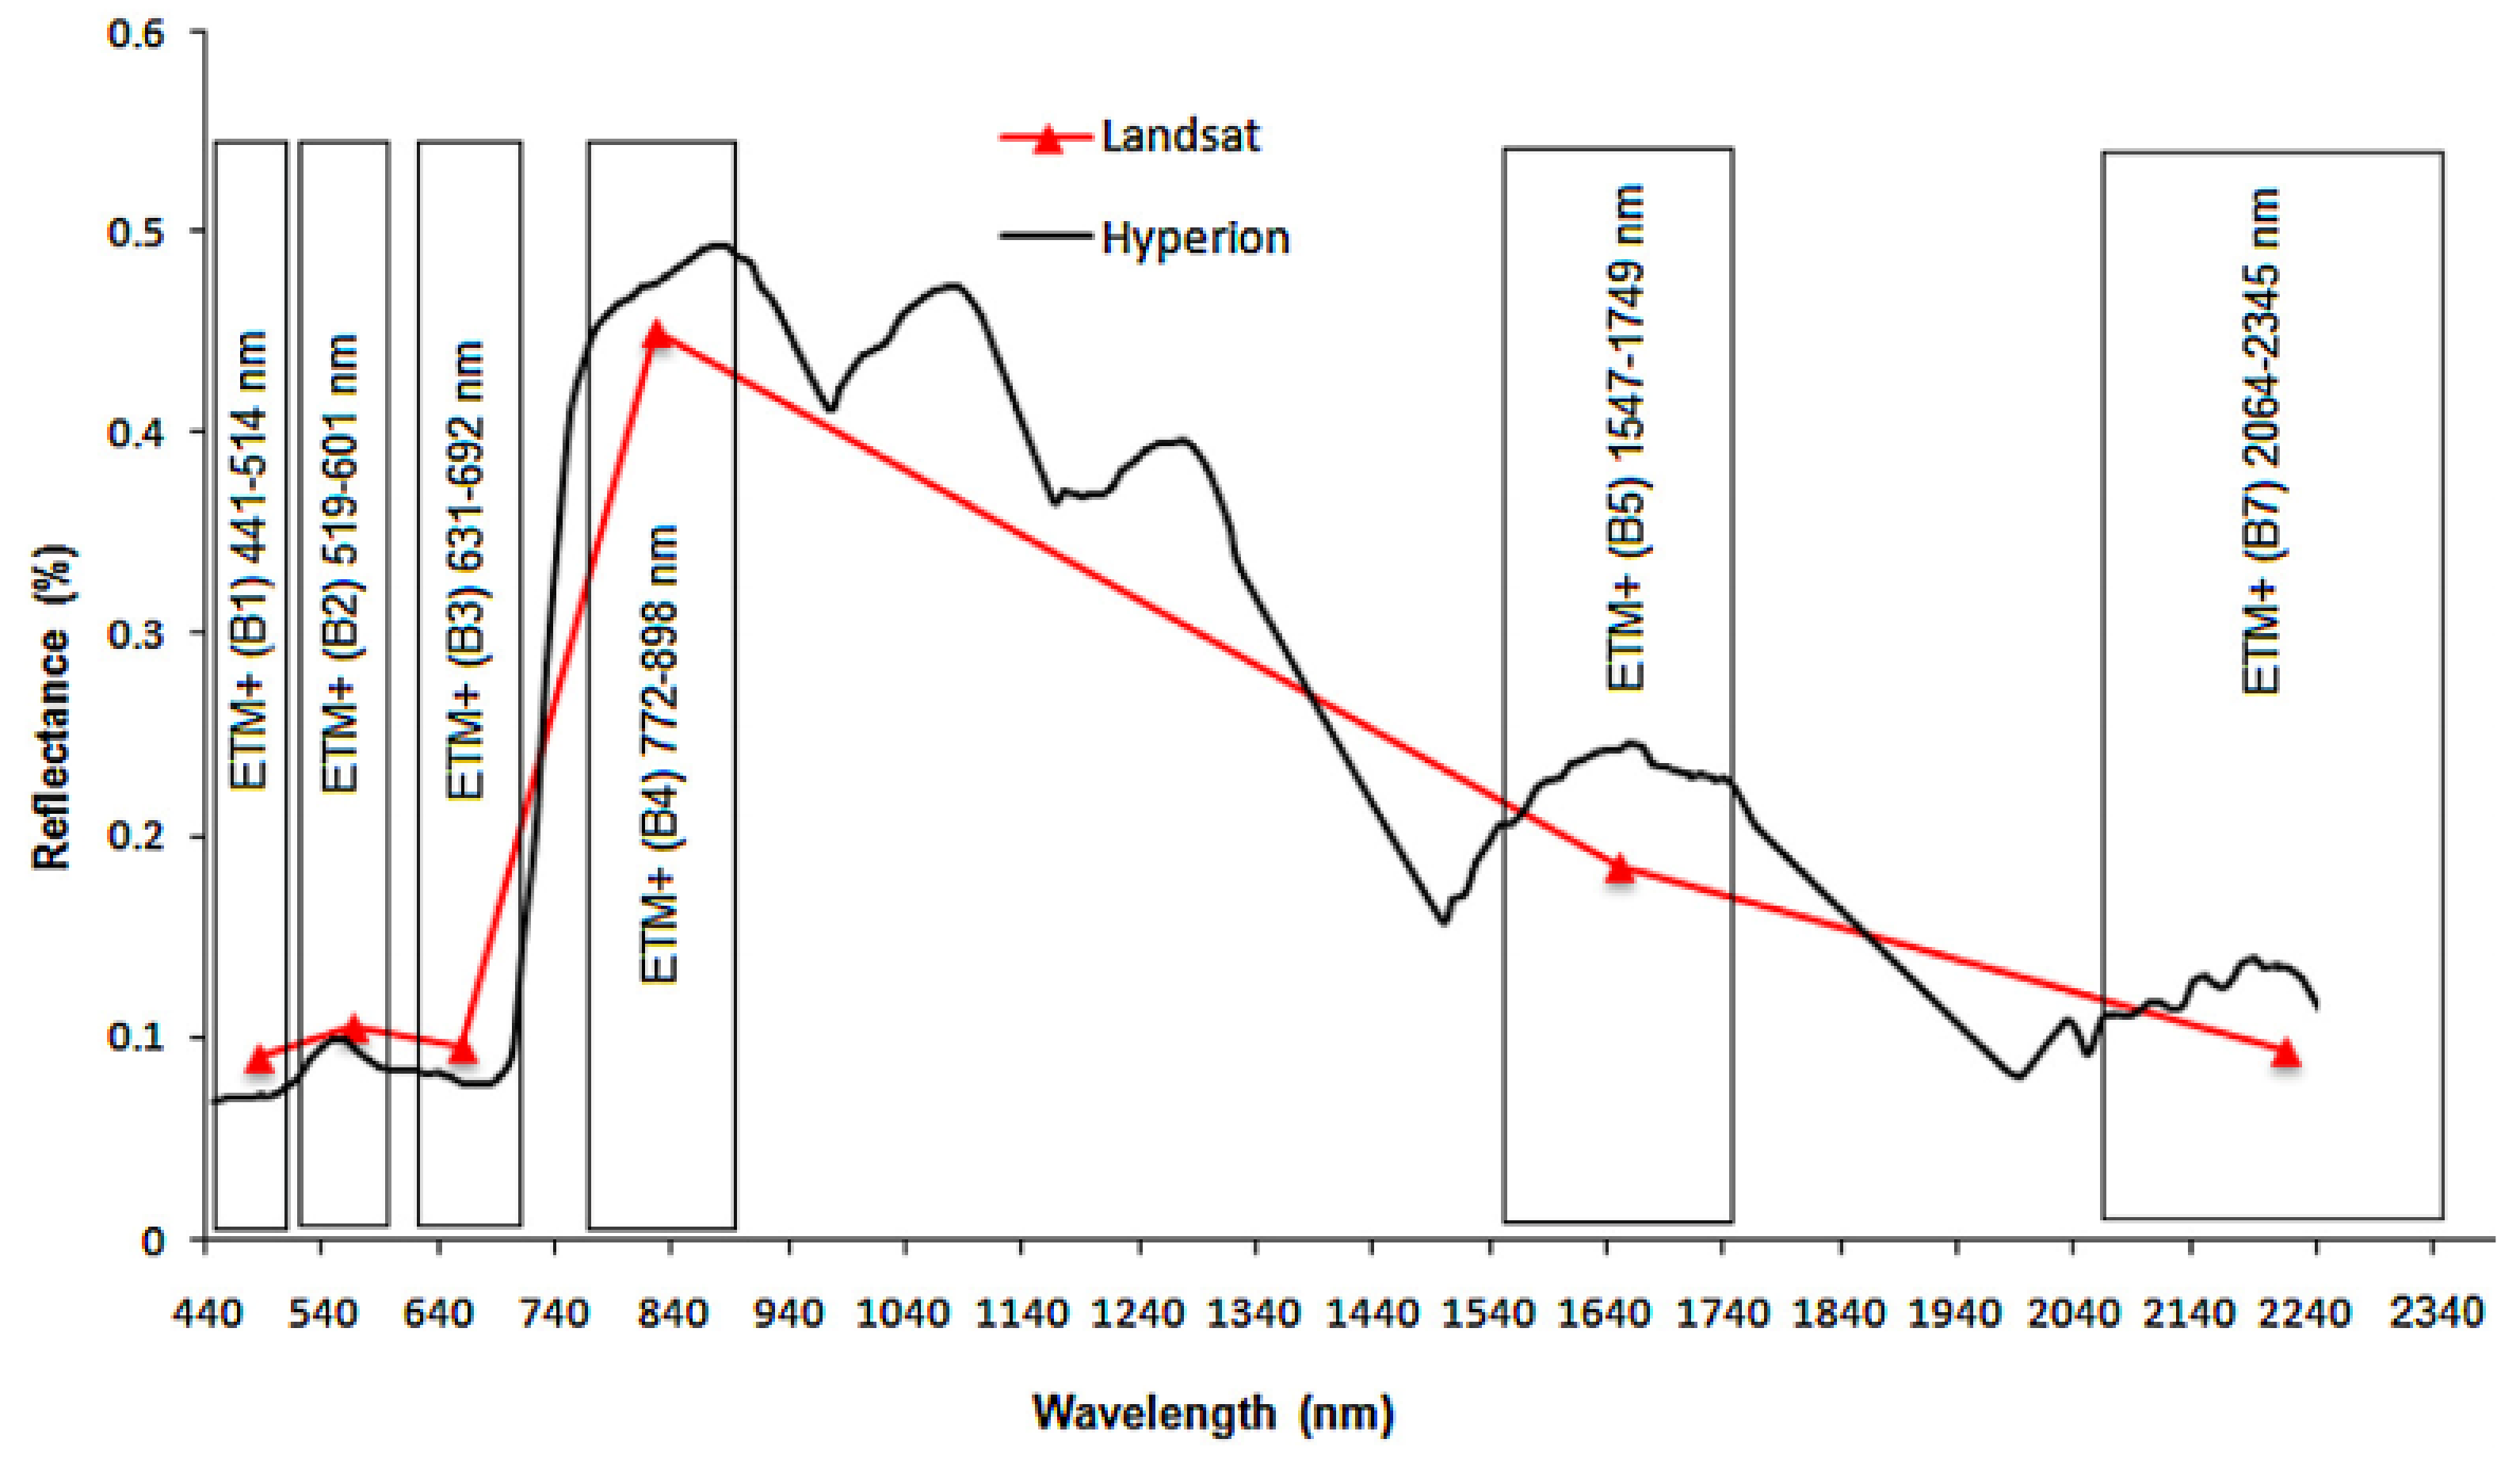
\includegraphics[width=0.8\textwidth]{img/4_marco_teorico/firma_cana.png}
    \label{fig:firma_cana}
    \begin{flushleft}
        \textit{Nota.} Extraído de \citet{hamzeh2016assessing}. 
        \vspace{-\baselineskip}
    \end{flushleft}
\end{figure}

\subsubsection{Cosecha y quema de caña de azúcar.}
\citet{pipicano_alisis_2022} mencionan que durante el proceso de cosecha del cultivo se tiene como residuos agrícolas a las hojas verdes y secas, raíces y el
cogollo de la planta (Figura \ref{fig:quema_cana}). En países como Brasil, Tailandia, Guatemala, Colombia, México y Costa Rica, la quema de estos residuos antes 
de la cosecha es una práctica común; en los Estados Unidos y Filipinas, los campos de caña de azúcar se queman antes o después de la cosecha. Sin embargo, en India y 
China la mayoría de los residuos de la caña de azúcar se queman en el campo después de la cosecha debido a la falta de técnicas de compostaje adecuadas 
\citep{world_bank_group,junpen_estimation_2020}.

\begin{figure}[H]
    \centering
    \caption{Partes de la caña de azúcar.}
    \includegraphics[width=0.4\textwidth]{img/4_marco_teorico/partes_caña.png}
    \label{fig:quema_cana}
    \begin{flushleft}
        \textit{Nota.} Extraído de \citet{pipicano_alisis_2022}. 
        \vspace{-\baselineskip}
    \end{flushleft}
\end{figure}
En el caso del Perú, se tiene la particularidad de permitir la cosecha de caña durante todo el año, 
sin una temporada específica de zafra a excepción de los meses de otoño (abril/mayo) que es cuando la sacarosa en la caña disminuye y se aprovecha
para realizar la Parada Anual, generalmente  en esta época donde practica el agoste entre los meses de abril a setiembre que consiste en la suspensión 
del riego para reducir el crecimiento de las hojas verdes, contribuyendo así a su secado y permitiendo la acumulación máxima de sacarosa durante el período de madurez.
\citep{helfgott_cultivo_2016}.

En cuanto a la etapa de cosecha y procesamiento, ambas se llevan a cabo dentro de un lapso no mayor a 48 horas. En este lapso se realiza la quema de caña de azúcar que es una labor crucial, antes de la cosecha, con el propósito de eliminar las hojas verdes y secas facilitando de esta manera el corte y transporte de la caña. 
Para llevar a cabo este procedimiento consideran factores como la distancia y la accesibilidad a las áreas, las condiciones 
de los campos, la proximidad a otros cultivos, viviendas y lugares habitados \citep[pp. 1530 - 1536]{casa_grande_saa_2018}. 

El proceso de quema inicia en sentido contrario a la dirección del viento para prevenir la propagación del fuego hacia áreas no deseadas, ejecutándose de manera uniforme y completa en toda el área asignada. 
En situaciones donde la quema inicial no logra eliminar completamente todo el material no deseado, se realiza una segunda quema o requema empleando el mismo equipo, lanzallamas o palos de paja con kerosene, 
y personal involucrado en la tarea \citep[pp. 434 - 436]{san_jacinto_2014}.

\subsubsection{Firma espectral de áreas quemadas.}
\citet{Pereira1999} indican que el infrarrojo cercano (NIR), comprendido en los rangos de longitud de onda ($0.7 - 1.3$ \mu m), es la región espectral donde la señal de las cicatrices de incendios recientes es más fuerte y generalmente se considera la mejor región espectral para la detección y mapeo de áreas quemadas especialmente cuando las 
cargas de combustible previas al incendio son elevadas y la combustión produce grandes cantidades de carbón vegetal que se depositan en el suelo. 

Dado que la vegetación verde es muy reflectante en el NIR, la quema suele 
causar disminuciones más o menos significativas de la reflectancia ya que tanto la vegetación verde y seca antes del incendio tienen reflectancias mayores que las quemas recientes, por lo que una caída en la reflectancia en el NIR es sistemático y sirve como un indicador confiable de áreas quemadas recientementes.

\citet{alcaras_2022} señalan que, tras un incendio, la reflectancia en el espectro del NIR disminuye considerablemente debido a la quema de la vegetación, mientras que la reflectancia en el espectro del SWIR aumenta como resultado de la pérdida de vegetación y, por ende, de agua (Figura \ref{fig:firma_espectral}). Asímismo, las regiones espectrales del Rojo y del Borde 
Rojo son cruciales para la detección de áreas quemadas, ya que están relacionadas con una fuerte absorción de clorofila en las plantas.

\begin{figure}[H]
    \centering
    \caption{Comparación de la respuesta espectral de la vegetación saludable y las áreas quemadas.}
    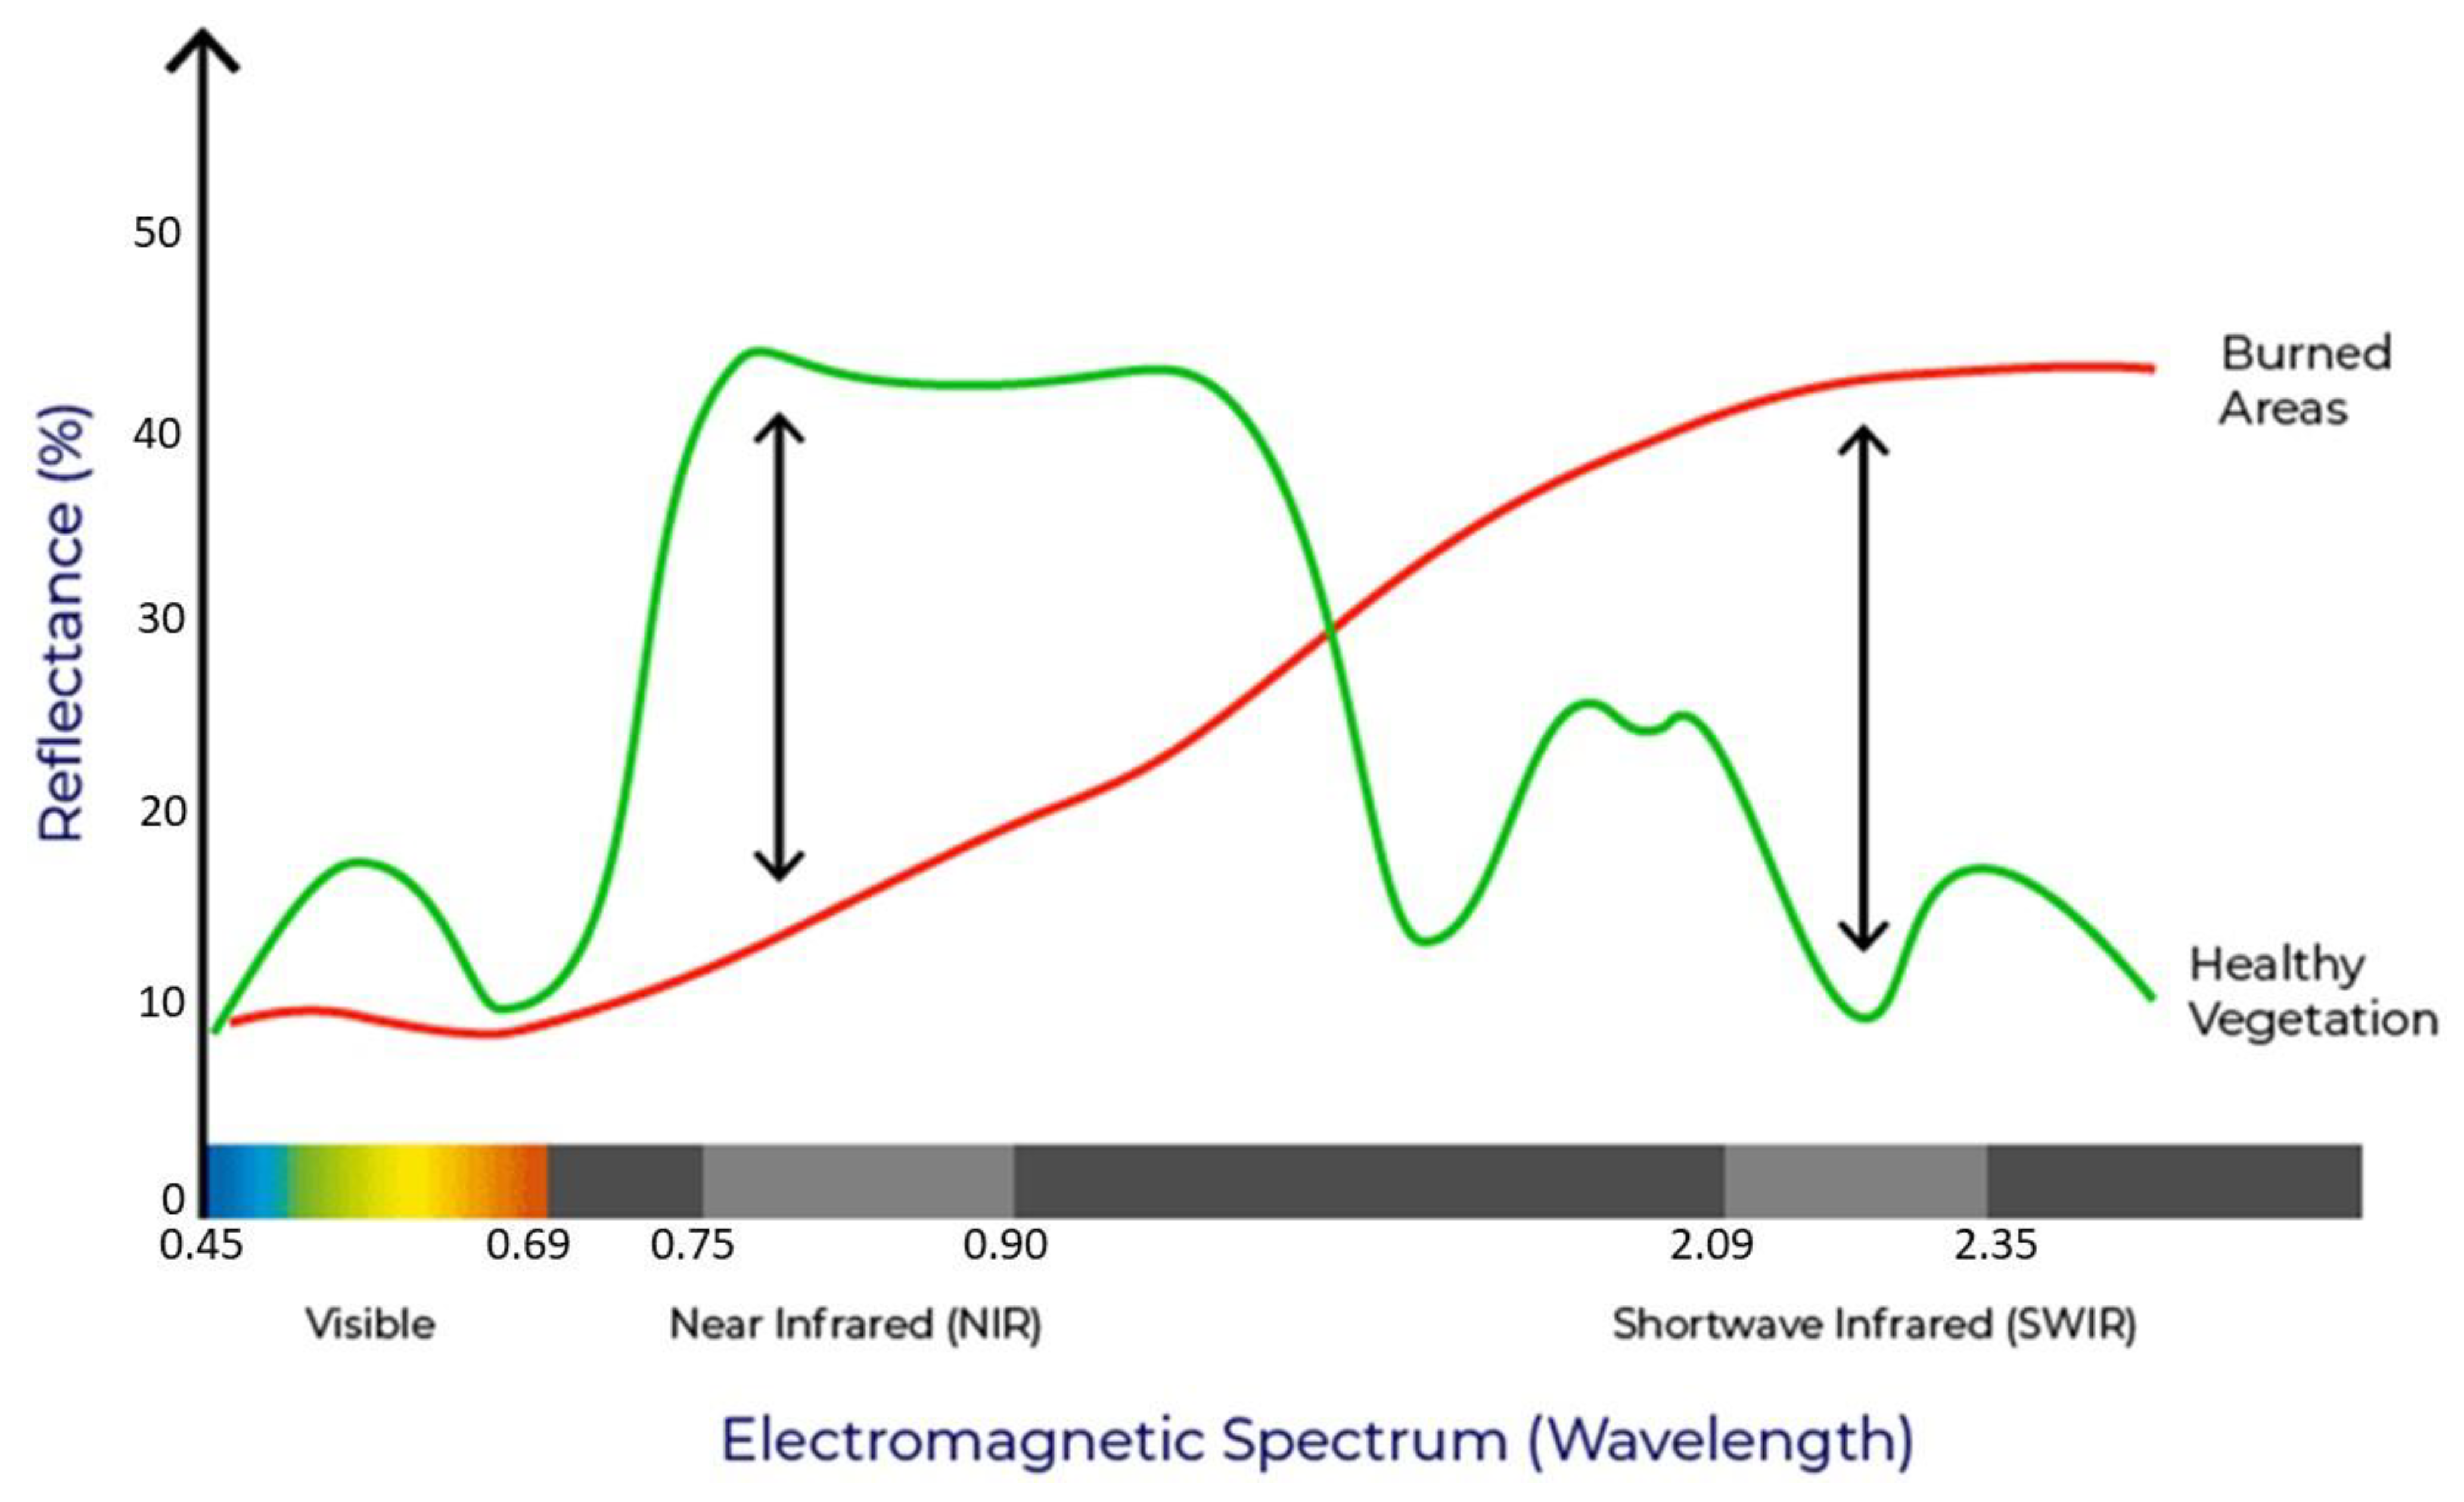
\includegraphics[width=0.6\textwidth]{img/4_marco_teorico/burned_areas_spectral.png}
    \label{fig:firma_espectral}
    \begin{flushleft}
        \textit{Nota.} Extraído de \citet{alcaras_2022}. 
        \vspace{-\baselineskip}
    \end{flushleft}
\end{figure}

